% Options for packages loaded elsewhere
\PassOptionsToPackage{unicode}{hyperref}
\PassOptionsToPackage{hyphens}{url}
%
\documentclass[
]{book}
\usepackage{lmodern}
\usepackage{amssymb,amsmath}
\usepackage{ifxetex,ifluatex}
\ifnum 0\ifxetex 1\fi\ifluatex 1\fi=0 % if pdftex
  \usepackage[T1]{fontenc}
  \usepackage[utf8]{inputenc}
  \usepackage{textcomp} % provide euro and other symbols
\else % if luatex or xetex
  \usepackage{unicode-math}
  \defaultfontfeatures{Scale=MatchLowercase}
  \defaultfontfeatures[\rmfamily]{Ligatures=TeX,Scale=1}
\fi
% Use upquote if available, for straight quotes in verbatim environments
\IfFileExists{upquote.sty}{\usepackage{upquote}}{}
\IfFileExists{microtype.sty}{% use microtype if available
  \usepackage[]{microtype}
  \UseMicrotypeSet[protrusion]{basicmath} % disable protrusion for tt fonts
}{}
\makeatletter
\@ifundefined{KOMAClassName}{% if non-KOMA class
  \IfFileExists{parskip.sty}{%
    \usepackage{parskip}
  }{% else
    \setlength{\parindent}{0pt}
    \setlength{\parskip}{6pt plus 2pt minus 1pt}}
}{% if KOMA class
  \KOMAoptions{parskip=half}}
\makeatother
\usepackage{xcolor}
\IfFileExists{xurl.sty}{\usepackage{xurl}}{} % add URL line breaks if available
\IfFileExists{bookmark.sty}{\usepackage{bookmark}}{\usepackage{hyperref}}
\hypersetup{
  pdftitle={Bioestadística Uno},
  pdfauthor={John Jairo Estrada Álvarez},
  hidelinks,
  pdfcreator={LaTeX via pandoc}}
\urlstyle{same} % disable monospaced font for URLs
\usepackage{color}
\usepackage{fancyvrb}
\newcommand{\VerbBar}{|}
\newcommand{\VERB}{\Verb[commandchars=\\\{\}]}
\DefineVerbatimEnvironment{Highlighting}{Verbatim}{commandchars=\\\{\}}
% Add ',fontsize=\small' for more characters per line
\usepackage{framed}
\definecolor{shadecolor}{RGB}{248,248,248}
\newenvironment{Shaded}{\begin{snugshade}}{\end{snugshade}}
\newcommand{\AlertTok}[1]{\textcolor[rgb]{0.94,0.16,0.16}{#1}}
\newcommand{\AnnotationTok}[1]{\textcolor[rgb]{0.56,0.35,0.01}{\textbf{\textit{#1}}}}
\newcommand{\AttributeTok}[1]{\textcolor[rgb]{0.77,0.63,0.00}{#1}}
\newcommand{\BaseNTok}[1]{\textcolor[rgb]{0.00,0.00,0.81}{#1}}
\newcommand{\BuiltInTok}[1]{#1}
\newcommand{\CharTok}[1]{\textcolor[rgb]{0.31,0.60,0.02}{#1}}
\newcommand{\CommentTok}[1]{\textcolor[rgb]{0.56,0.35,0.01}{\textit{#1}}}
\newcommand{\CommentVarTok}[1]{\textcolor[rgb]{0.56,0.35,0.01}{\textbf{\textit{#1}}}}
\newcommand{\ConstantTok}[1]{\textcolor[rgb]{0.00,0.00,0.00}{#1}}
\newcommand{\ControlFlowTok}[1]{\textcolor[rgb]{0.13,0.29,0.53}{\textbf{#1}}}
\newcommand{\DataTypeTok}[1]{\textcolor[rgb]{0.13,0.29,0.53}{#1}}
\newcommand{\DecValTok}[1]{\textcolor[rgb]{0.00,0.00,0.81}{#1}}
\newcommand{\DocumentationTok}[1]{\textcolor[rgb]{0.56,0.35,0.01}{\textbf{\textit{#1}}}}
\newcommand{\ErrorTok}[1]{\textcolor[rgb]{0.64,0.00,0.00}{\textbf{#1}}}
\newcommand{\ExtensionTok}[1]{#1}
\newcommand{\FloatTok}[1]{\textcolor[rgb]{0.00,0.00,0.81}{#1}}
\newcommand{\FunctionTok}[1]{\textcolor[rgb]{0.00,0.00,0.00}{#1}}
\newcommand{\ImportTok}[1]{#1}
\newcommand{\InformationTok}[1]{\textcolor[rgb]{0.56,0.35,0.01}{\textbf{\textit{#1}}}}
\newcommand{\KeywordTok}[1]{\textcolor[rgb]{0.13,0.29,0.53}{\textbf{#1}}}
\newcommand{\NormalTok}[1]{#1}
\newcommand{\OperatorTok}[1]{\textcolor[rgb]{0.81,0.36,0.00}{\textbf{#1}}}
\newcommand{\OtherTok}[1]{\textcolor[rgb]{0.56,0.35,0.01}{#1}}
\newcommand{\PreprocessorTok}[1]{\textcolor[rgb]{0.56,0.35,0.01}{\textit{#1}}}
\newcommand{\RegionMarkerTok}[1]{#1}
\newcommand{\SpecialCharTok}[1]{\textcolor[rgb]{0.00,0.00,0.00}{#1}}
\newcommand{\SpecialStringTok}[1]{\textcolor[rgb]{0.31,0.60,0.02}{#1}}
\newcommand{\StringTok}[1]{\textcolor[rgb]{0.31,0.60,0.02}{#1}}
\newcommand{\VariableTok}[1]{\textcolor[rgb]{0.00,0.00,0.00}{#1}}
\newcommand{\VerbatimStringTok}[1]{\textcolor[rgb]{0.31,0.60,0.02}{#1}}
\newcommand{\WarningTok}[1]{\textcolor[rgb]{0.56,0.35,0.01}{\textbf{\textit{#1}}}}
\usepackage{longtable,booktabs}
% Correct order of tables after \paragraph or \subparagraph
\usepackage{etoolbox}
\makeatletter
\patchcmd\longtable{\par}{\if@noskipsec\mbox{}\fi\par}{}{}
\makeatother
% Allow footnotes in longtable head/foot
\IfFileExists{footnotehyper.sty}{\usepackage{footnotehyper}}{\usepackage{footnote}}
\makesavenoteenv{longtable}
\usepackage{graphicx,grffile}
\makeatletter
\def\maxwidth{\ifdim\Gin@nat@width>\linewidth\linewidth\else\Gin@nat@width\fi}
\def\maxheight{\ifdim\Gin@nat@height>\textheight\textheight\else\Gin@nat@height\fi}
\makeatother
% Scale images if necessary, so that they will not overflow the page
% margins by default, and it is still possible to overwrite the defaults
% using explicit options in \includegraphics[width, height, ...]{}
\setkeys{Gin}{width=\maxwidth,height=\maxheight,keepaspectratio}
% Set default figure placement to htbp
\makeatletter
\def\fps@figure{htbp}
\makeatother
\setlength{\emergencystretch}{3em} % prevent overfull lines
\providecommand{\tightlist}{%
  \setlength{\itemsep}{0pt}\setlength{\parskip}{0pt}}
\setcounter{secnumdepth}{5}
\usepackage{booktabs}
\usepackage{booktabs}
\usepackage{longtable}

\ifxetex
  \usepackage{letltxmacro}
  \setlength{\XeTeXLinkMargin}{1pt}
  \LetLtxMacro\SavedIncludeGraphics\includegraphics
  \def\includegraphics#1#{% #1 catches optional stuff (star/opt. arg.)
    \IncludeGraphicsAux{#1}%
  }%
  \newcommand*{\IncludeGraphicsAux}[2]{%
    \XeTeXLinkBox{%
      \SavedIncludeGraphics#1{#2}%
    }%
  }%
\fi
\usepackage[]{natbib}
\bibliographystyle{apalike}

\title{Bioestadística Uno}
\author{John Jairo Estrada Álvarez}
\date{2021-08-09}

\usepackage{amsthm}
\newtheorem{theorem}{Teorema}[chapter]
\newtheorem{lemma}{Lema}[chapter]
\newtheorem{corollary}{Corolario}[chapter]
\newtheorem{proposition}{Proposición}[chapter]
\newtheorem{conjecture}{Conjecture}[chapter]
\theoremstyle{definition}
\newtheorem{definition}{Definición}[chapter]
\theoremstyle{definition}
\newtheorem{example}{Ejemplo}[chapter]
\theoremstyle{definition}
\newtheorem{exercise}{Ejercicio}[chapter]
\theoremstyle{definition}
\newtheorem{hypothesis}{Hypothesis}[chapter]
\theoremstyle{remark}
\newtheorem*{remark}{Nota:}
\newtheorem*{solution}{Solución}
\begin{document}
\maketitle

{
\setcounter{tocdepth}{1}
\tableofcontents
}
\hypertarget{prerrequisitos}{%
\chapter{Prerrequisitos}\label{prerrequisitos}}

\hypertarget{objetivos-especuxedficos}{%
\section{Objetivos específicos}\label{objetivos-especuxedficos}}

\begin{itemize}
\tightlist
\item
  Describir los conceptos de población, muestra, variables y datos, así como también,
  discriminar entre los diversos tipos de variables.
\item
  Producir una descripción tabular y gráfica de los datos de la muestra y resumir tales datos
  mediante estadísticos de tendencia central, dispersión y distribución, todo esto apoyado en
  un programa computacional de estadística.
\item
  Aprender el concepto de probabilidad considerando la misma como una estrategia para
  cuantificar fenómenos aleatorios y aplicar la teoría matemática básica sobre el cálculo de
  probabilidades.
\item
  Explicar el concepto de variable aleatoria y de modelo de distribución de probabilidad, así
  como también, discriminar entre diversos tipos de variables aleatorias y sus modelos
  asociados (por ejemplo, Binomial, Normal, Poisson, etc.)
\end{itemize}

\hypertarget{fechas-de-evaluaciuxf3n-segundo-semestre-2021}{%
\section{Fechas de Evaluación segundo semestre 2021}\label{fechas-de-evaluaciuxf3n-segundo-semestre-2021}}

\begin{itemize}
\item
  Primer parcial (25 \(\%\)) - \textbf{Fecha: Viernes \(13\) de Agosto}
\item
  Segundo Parcial (25 \(\%\)) - \textbf{Fecha: Viernes \(10\) de Septiembre}
\item
  Tercer Parcial (25 \(\%\)) - \textbf{Fecha: Viernes \(8\) de Octubre}
\item
  Cuarto Parcial (ó Parcial Final) (25 \(\%\)) - \textbf{Fecha: Viernes \(3\) de Noviembre}
\end{itemize}

\begin{verbatim}
## ~~ Package calendR
## Visit https://r-coder.com/ for R tutorials ~~
\end{verbatim}

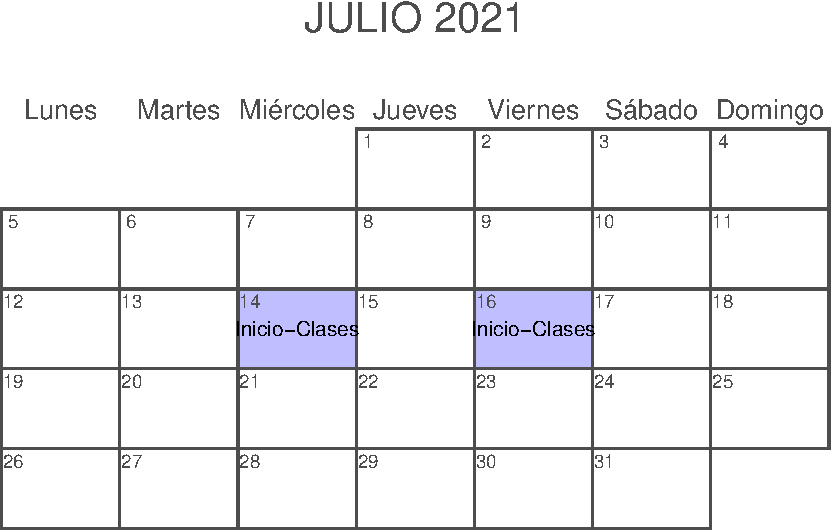
\includegraphics{BioestadisticaUnoUCES2021_files/figure-latex/unnamed-chunk-1-1.pdf}

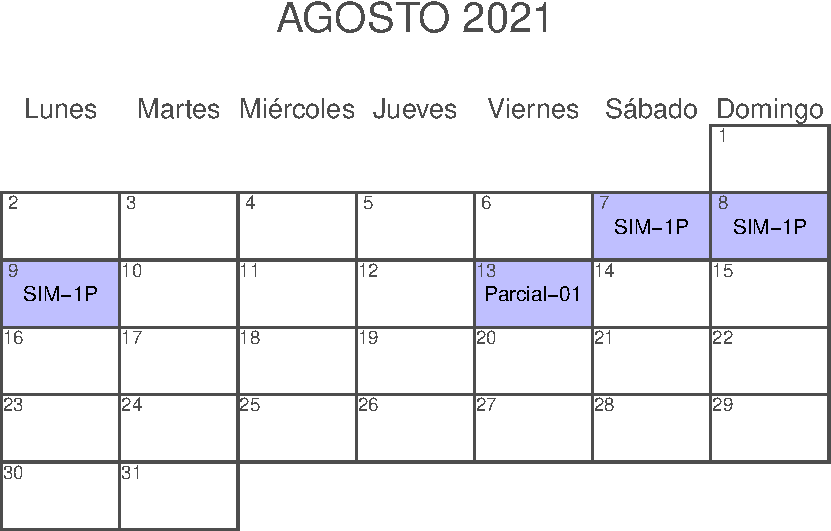
\includegraphics{BioestadisticaUnoUCES2021_files/figure-latex/unnamed-chunk-2-1.pdf}

\hypertarget{bibliografuxeda-del-curso}{%
\section{Bibliografía del curso}\label{bibliografuxeda-del-curso}}

\begin{itemize}
\item
  Samuels, M., Witmer, J., \& Schaffner, A. (2012). Statistics for the life sciences (4 ed.).
  Boston: Pearson Education.
\item
  Milton, J. S. (2001). Estadística para la biología y ciencias de la salud (3 ed.). Madrid:
  McGraw- Hill/Interamericana.
\item
  Daniel, W. W. 2004. Bioestadística. Base para el análisis de las ciencias de la salud. 4era. Ed.
  Limusa Wiley Noriega Editores. México.
\item
  Johnson, R. A. \& Bhattacharyya, G. K. (2010). Statistics. Principles and Methods (6 ed.). New
  York: John Wiley and Sons, Inc
\item
  Zar, J. (1999). Biostatistical analysis (5 ed.). Prentice hall Upper Saddle River, NJ.
\item
  Zuur, A., Ieno, E., \& Meesters, E. (2009). A Beginner's Guide to R. Springer.
\end{itemize}

\hypertarget{intro}{%
\chapter{Introduction}\label{intro}}

\hypertarget{conceptos-introductorios}{%
\section{Conceptos Introductorios}\label{conceptos-introductorios}}

\hypertarget{de-donde-viene-la-palabra-estadux131ux301stica-y-que-significa}{%
\subsection{\texorpdfstring{\textbf{¿De donde viene la palabra estadı́stica y que significa?}}{¿De donde viene la palabra estadı́stica y que significa?}}\label{de-donde-viene-la-palabra-estadux131ux301stica-y-que-significa}}

\begin{itemize}
\tightlist
\item
  \textbf{Respuesta}:
  Viene del latı́n status.
  Significa estado.
  La estadı́stica comenzó colectando\\
  y resumiendo información (o datos) sobre el estado.
  Aún hoy dı́a, un segmento grande del
  público en general piensa en la
  estadı́stica como un sinónimo de datos,
  tablas y gráficas.
\end{itemize}

A comienzos del siglo XX algunos matemáticos como Karl Pearson
y Ronald A Fisher realizaron avances matemáticos importantes que
posicionaron la Estadı́stica como una ciencia independiente para
ser usada en el análisis e interpretación de los datos en la
investigación cientı́fica.

\begin{figure}

{\centering 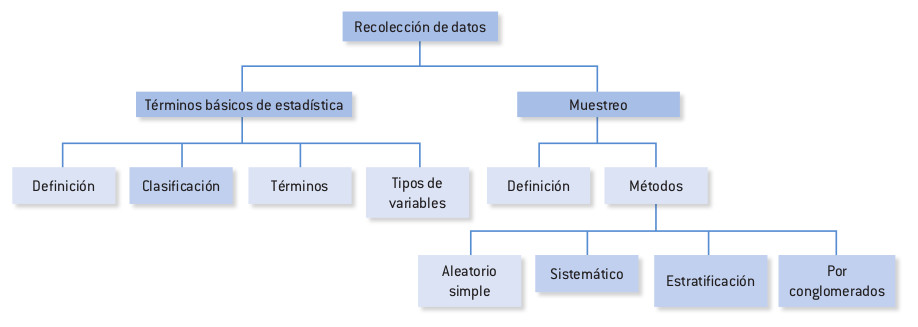
\includegraphics[width=0.85\linewidth]{/home/john/Documentos/MatematicasBioEstadisticaV1/BioestadisticaUnoUCES2021/images/EstadisticaColeccion1} 

}

\caption{Fundamentos de la estadística [Imagen tomada de [@gutierrez2012probabilidad] pág $4$]}\label{fig:Estadistica1}
\end{figure}

\hypertarget{quuxe9-es-la-estaduxedstica}{%
\subsection{\texorpdfstring{\textbf{¿Qué es la estadística?}}{¿Qué es la estadística?}}\label{quuxe9-es-la-estaduxedstica}}

\begin{itemize}
\item
  \textbf{Respuesta}:
  Es el arte de la decisión frente a la
  incertidumbre.
  Milton (2001,pág. 1)
  Es la disciplina que ofrece un conjunto
  de técnicas para diseñar el proceso de
  colectar, resumir e interpretar datos, ası́
  como también, obtener conclusiones o
  generalidades a partir de ellos.
  Johnnson \& Bahttachaaryya (1996,
  pág. 3)
\item
  \textbf{Respuesta}:(\citet{lind2012estadistica})
  Ciencia que recoge, organiza, presenta, analiza e interpreta datos con el find e proporcionar una toma
  de decisiones más eficaz.
\item
  \textbf{Respuesta}:(\citet{martinez2012estadistica})
  Sistema o método usado en la recolección, organización, análisis y descripción numérica de la información. También se puede decir que la estadística estudia el comportamiento de hechos o fenómenos de grupo.
\end{itemize}

\begin{figure}

{\centering 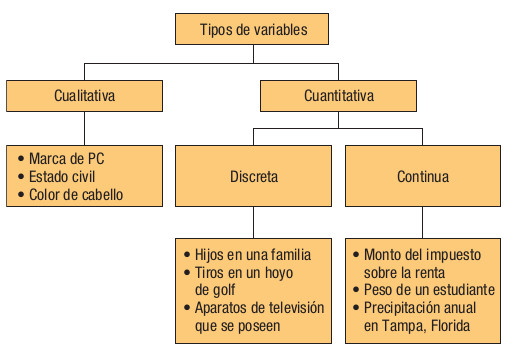
\includegraphics[width=0.65\linewidth]{/home/john/Documentos/MatematicasBioEstadisticaV1/BioestadisticaUnoUCES2021/images/TIPOSDEVARIABLE1} 

}

\caption{Resumen tipos de variables [Imagen tomada de [@lind2012estadistica] pág $9$]}\label{fig:TipoVariable1}
\end{figure}

\hypertarget{quuxe9-es-una-variable}{%
\subsection{\texorpdfstring{\textbf{¿Qué es una variable?}}{¿Qué es una variable?}}\label{quuxe9-es-una-variable}}

\begin{itemize}
\tightlist
\item
  \textbf{Respuesta}:
  Una variable representa una
  caracterı́stica o rasgo compartido por un
  grupo de elementos (objetos o
  entidades), que toma más de un posible
  valor (numérico o de texto) entre los
  elementos del grupo.
\end{itemize}

\hypertarget{variable-categuxf3rica-uxf3-cualitativa}{%
\subsection{\texorpdfstring{\textbf{Variable categórica (ó cualitativa)}}{Variable categórica (ó cualitativa)}}\label{variable-categuxf3rica-uxf3-cualitativa}}

\begin{itemize}
\item
  Si sus valores no se pueden asociar naturalmente a un número
  (no se puede hacer operaciones aritméticas con ellos)

  \begin{enumerate}
  \def\labelenumi{\arabic{enumi}.}
  \tightlist
  \item
    \textbf{Nominales}: Si sus valores no tiene un orden natural

    \begin{enumerate}
    \def\labelenumii{\alph{enumii}.}
    \tightlist
    \item
      Ejemplos: Sexo, rasgos fenotípicos y genotípicos, Fumar Si/No, Color, Nacionalidad, etc
    \end{enumerate}
  \item
    \textbf{Ordinales}: Si sus valores se pueden ordenar de forma natural

    \begin{enumerate}
    \def\labelenumii{\alph{enumii}.}
    \setcounter{enumii}{1}
    \tightlist
    \item
      Ejemplos: Mejora de un tratamiento, resistencia al dolor, grado de felicidad, etc
    \end{enumerate}
  \end{enumerate}
\end{itemize}

\hypertarget{variable-cuantitativa-si-sus-valores-son-numuxe9ricos-si-se-pueden-hacer-operaciones-aritmuxe9ticas-con-ellos.}{%
\subsection{\texorpdfstring{\textbf{Variable cuantitativa}: Si sus valores son numéricos (si se pueden hacer operaciones aritméticas con ellos).}{Variable cuantitativa: Si sus valores son numéricos (si se pueden hacer operaciones aritméticas con ellos).}}\label{variable-cuantitativa-si-sus-valores-son-numuxe9ricos-si-se-pueden-hacer-operaciones-aritmuxe9ticas-con-ellos.}}

\begin{itemize}
\tightlist
\item
  \textbf{Continuos}: Si toma valores en una escala continua en los números reales.
\item
  \textbf{Discretos}: Si toma valores enteros. Por lo general resultan del proceso de contar.
\end{itemize}

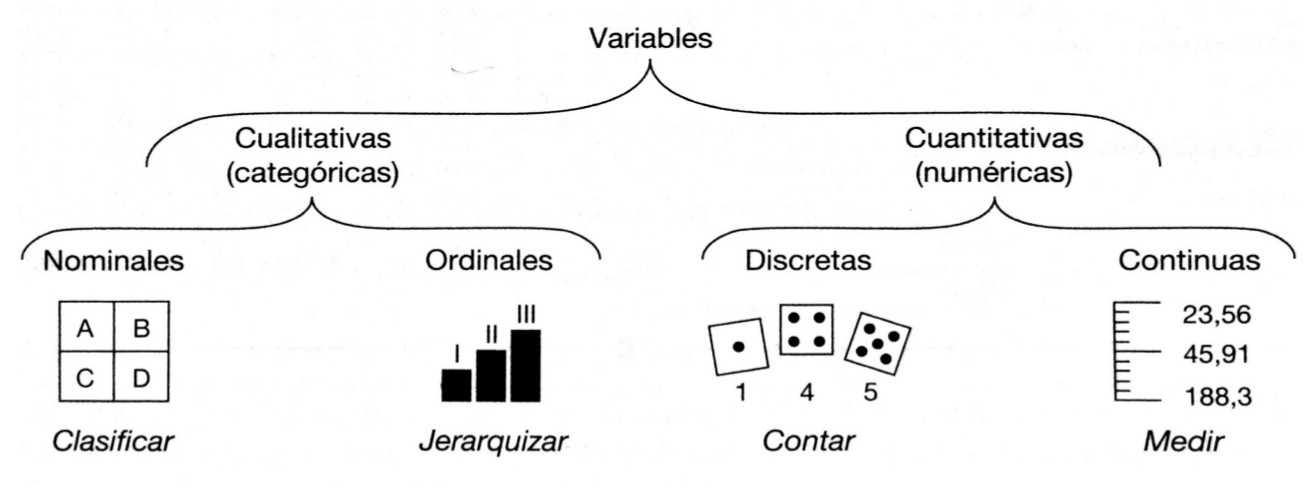
\includegraphics[width=0.75\textwidth,height=\textheight]{/home/john/Documentos/MatematicasBioEstadisticaV1/BioestadisticaUnoUCES2021/images/GRAFIACAtipodeVariables2.jpg}

\hypertarget{quuxe9-es-un-dato}{%
\subsection{\texorpdfstring{\textbf{¿Qué es un dato?}}{¿Qué es un dato?}}\label{quuxe9-es-un-dato}}

\begin{itemize}
\tightlist
\item
  \textbf{Respuesta}:
  Un dato es el resultado de realizar una
  observación o medición sobre un
  elemento del grupo de interés. Se puede
  tener un dato en una sola variable o en
  más de una variable.
\end{itemize}

El término en plural datos o conjuntos
de datos hace referencia al conjunto de
observaciones realizadas sobre cada uno
de los elementos del grupo de interés

\hypertarget{quuxe9-es-una-unidad-de-observaciuxf3n}{%
\subsection{\texorpdfstring{\textbf{¿Qué es una unidad de observación?}}{¿Qué es una unidad de observación?}}\label{quuxe9-es-una-unidad-de-observaciuxf3n}}

\begin{itemize}
\tightlist
\item
  \textbf{Respuesta}: Es un elemento ó persona a la cual se le miden una (ó más) variables sobre ella.
\end{itemize}

\hypertarget{quuxe9-es-una-poblaciuxf3n}{%
\subsection{\texorpdfstring{\textbf{¿Qué es una población?}}{¿Qué es una población?}}\label{quuxe9-es-una-poblaciuxf3n}}

\begin{itemize}
\tightlist
\item
  \textbf{Respuesta}: Una población es la colección entera de
  unidades de observación que se desea
  estudiar.
  Por lo general, tal colección esta
  definida por ciertas condiciones fı́sicas,
  biológicas, espaciales o temporales
  establecidas por los objetivos de la
  investigación.
  En muchas ocasiones, las poblaciones
  son demasiado grandes o incluso
  infinitas
\end{itemize}

\hypertarget{quuxe9-es-una-muestra}{%
\subsection{\texorpdfstring{\textbf{¿Qué es una muestra?}}{¿Qué es una muestra?}}\label{quuxe9-es-una-muestra}}

\begin{itemize}
\item
  \textbf{Respuesta}: Una muestra es un subconjunto de
  elementos de la población. La muestra
  se obtiene para generalizar a toda la
  población lo observado en la muestra.
  Cualidades de la muestra

  \begin{enumerate}
  \def\labelenumi{\alph{enumi}.}
  \tightlist
  \item
    Representativa de toda la población
  \item
    Tomada al azar (es decir todos los elementos de la población tienen la misma probabilidad)
  \end{enumerate}
\end{itemize}

\begin{figure}

{\centering 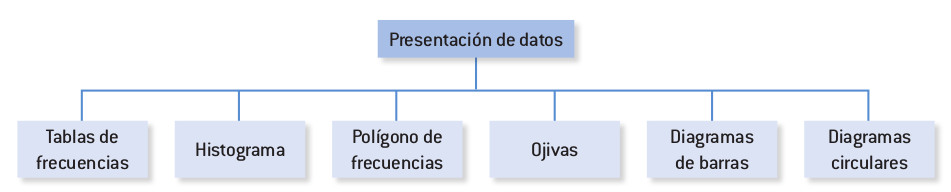
\includegraphics[width=0.65\linewidth]{/home/john/Documentos/MatematicasBioEstadisticaV1/BioestadisticaUnoUCES2021/images/GRAFICOresumenPresentacionDatos} 

}

\caption{Presentación de datos [Imagen tomada de [@gutierrez2012probabilidad] pág $9$]}\label{fig:TipoDatos1}
\end{figure}

\hypertarget{estaduxedstica-descriptiva}{%
\chapter{Estadística descriptiva}\label{estaduxedstica-descriptiva}}

\hypertarget{quuxe9-es-la-estraduxedstica-descriptiva}{%
\section{Qué es la Estradística descriptiva?}\label{quuxe9-es-la-estraduxedstica-descriptiva}}

Es el conjunto de técnicas para organizar y describir un conjunto de datos (muestra)
utilizando métodos numéricos y gráficos que resumen y presentan la información contenida
en ellos.

\textbf{Ejercicios para entrenar el manejo datos}

\begin{itemize}
\tightlist
\item
  Ejemplo3
\end{itemize}

\hypertarget{los-aspectos-importantes-de-los-datos}{%
\subsection{Los aspectos importantes de los datos}\label{los-aspectos-importantes-de-los-datos}}

\begin{enumerate}
\def\labelenumi{\arabic{enumi}.}
\tightlist
\item
  \textbf{Destribución de frecuencias}
\end{enumerate}

Cómo están repartidos o distribuidos los datos en el rango de valores de la variable evaluada?

\begin{itemize}
\tightlist
\item
  Ejemplo1
\end{itemize}

Se entrevistó 20 jóvenes para conocer el número de refrescos de cola que beben al día. Las respuestas obtenidas son los siguientes:

\begin{equation}
\begin{matrix}
5 & 2 & 2 & 4 & 5\\
1 & 1 & 4 & 2 & 1\\
3 & 5 & 1 & 0 & 5\\ 
0 & 3 & 2 & 3 & 4
\end{matrix}
\end{equation}

\hypertarget{frecuencia-relativa}{%
\subsection{Frecuencia relativa}\label{frecuencia-relativa}}

\begin{Shaded}
\begin{Highlighting}[]
\NormalTok{Pc <-}\StringTok{ }\KeywordTok{c}\NormalTok{(}\DecValTok{5}\NormalTok{,}\DecValTok{1}\NormalTok{,}\DecValTok{3}\NormalTok{,}\DecValTok{0}\NormalTok{,}\DecValTok{2}\NormalTok{,}\DecValTok{1}\NormalTok{,}\DecValTok{5}\NormalTok{,}\DecValTok{3}\NormalTok{,}\DecValTok{2}\NormalTok{,}\DecValTok{4}\NormalTok{,}\DecValTok{1}\NormalTok{,}\DecValTok{2}\NormalTok{,}\DecValTok{4}\NormalTok{,}\DecValTok{2}\NormalTok{,}\DecValTok{0}\NormalTok{,}\DecValTok{3}\NormalTok{,}\DecValTok{5}\NormalTok{,}\DecValTok{1}\NormalTok{,}\DecValTok{5}\NormalTok{,}\DecValTok{4}\NormalTok{)}
\NormalTok{Tabla1 <-}\StringTok{ }\KeywordTok{as.data.frame}\NormalTok{(}\KeywordTok{sort}\NormalTok{(}\KeywordTok{table}\NormalTok{(}\DataTypeTok{TC3 =}\NormalTok{Pc),}\DataTypeTok{decreasing =}\NormalTok{ T))}
\NormalTok{Tabla2 <-}\StringTok{ }\KeywordTok{transform}\NormalTok{(Tabla1, }\DataTypeTok{FreAc =} \KeywordTok{cumsum}\NormalTok{(Freq))}
\NormalTok{Tabla3 <-}\StringTok{ }\KeywordTok{transform}\NormalTok{(Tabla2,}\DataTypeTok{Rel =} \KeywordTok{round}\NormalTok{(}\KeywordTok{prop.table}\NormalTok{(Freq),}\DecValTok{3}\NormalTok{))}
\NormalTok{knitr}\OperatorTok{::}\KeywordTok{kable}\NormalTok{(}
\NormalTok{Tabla3,}
\DataTypeTok{caption =} \StringTok{'Frecuencia Relativa'}\NormalTok{,}
  \DataTypeTok{booktabs =} \OtherTok{TRUE}
\NormalTok{)}
\end{Highlighting}
\end{Shaded}

\begin{table}

\caption{\label{tab:Tabla1}Frecuencia Relativa}
\centering
\begin{tabular}[t]{lrrr}
\toprule
TC3 & Freq & FreAc & Rel\\
\midrule
1 & 4 & 4 & 0.20\\
2 & 4 & 8 & 0.20\\
5 & 4 & 12 & 0.20\\
3 & 3 & 15 & 0.15\\
4 & 3 & 18 & 0.15\\
\addlinespace
0 & 2 & 20 & 0.10\\
\bottomrule
\end{tabular}
\end{table}

\hypertarget{frecuencia-relativa-y-acumulada}{%
\subsection{Frecuencia relativa y acumulada}\label{frecuencia-relativa-y-acumulada}}

\begin{Shaded}
\begin{Highlighting}[]
\NormalTok{Pc <-}\StringTok{ }\KeywordTok{c}\NormalTok{(}\DecValTok{5}\NormalTok{,}\DecValTok{1}\NormalTok{,}\DecValTok{3}\NormalTok{,}\DecValTok{0}\NormalTok{,}\DecValTok{2}\NormalTok{,}\DecValTok{1}\NormalTok{,}\DecValTok{5}\NormalTok{,}\DecValTok{3}\NormalTok{,}\DecValTok{2}\NormalTok{,}\DecValTok{4}\NormalTok{,}\DecValTok{1}\NormalTok{,}\DecValTok{2}\NormalTok{,}\DecValTok{4}\NormalTok{,}\DecValTok{2}\NormalTok{,}\DecValTok{0}\NormalTok{,}\DecValTok{3}\NormalTok{,}\DecValTok{5}\NormalTok{,}\DecValTok{1}\NormalTok{,}\DecValTok{5}\NormalTok{,}\DecValTok{4}\NormalTok{)}
\NormalTok{Tabla1 <-}\StringTok{ }\KeywordTok{as.data.frame}\NormalTok{(}\KeywordTok{sort}\NormalTok{(}\KeywordTok{table}\NormalTok{(}\DataTypeTok{TC3 =}\NormalTok{Pc),}\DataTypeTok{decreasing =}\NormalTok{ T))}
\NormalTok{Tabla2 <-}\StringTok{ }\KeywordTok{transform}\NormalTok{(Tabla1, }\DataTypeTok{FreAc =} \KeywordTok{cumsum}\NormalTok{(Freq))}
\NormalTok{Tabla3 <-}\StringTok{ }\KeywordTok{transform}\NormalTok{(Tabla2,}\DataTypeTok{Rel =} \KeywordTok{round}\NormalTok{(}\KeywordTok{prop.table}\NormalTok{(Freq),}\DecValTok{3}\NormalTok{))}
\NormalTok{Tabla4 <-}\StringTok{ }\KeywordTok{transform}\NormalTok{(Tabla3,}\DataTypeTok{RelAc =} \KeywordTok{round}\NormalTok{(}\KeywordTok{cumsum}\NormalTok{(}\KeywordTok{prop.table}\NormalTok{(Freq)),}\DecValTok{3}\NormalTok{))}
\NormalTok{knitr}\OperatorTok{::}\KeywordTok{kable}\NormalTok{(}
\NormalTok{Tabla4 , }\DataTypeTok{caption =} \StringTok{'Frecuencia relativa y acumulada'}\NormalTok{,}
  \DataTypeTok{booktabs =} \OtherTok{TRUE}
\NormalTok{)}
\end{Highlighting}
\end{Shaded}

\begin{table}

\caption{\label{tab:Tabla2}Frecuencia relativa y acumulada}
\centering
\begin{tabular}[t]{lrrrr}
\toprule
TC3 & Freq & FreAc & Rel & RelAc\\
\midrule
1 & 4 & 4 & 0.20 & 0.20\\
2 & 4 & 8 & 0.20 & 0.40\\
5 & 4 & 12 & 0.20 & 0.60\\
3 & 3 & 15 & 0.15 & 0.75\\
4 & 3 & 18 & 0.15 & 0.90\\
\addlinespace
0 & 2 & 20 & 0.10 & 1.00\\
\bottomrule
\end{tabular}
\end{table}

Comando para obtener el Rango de una variable: Ej obtener el rango de la variable EDAD

\begin{Shaded}
\begin{Highlighting}[]
\NormalTok{Pc <-}\StringTok{ }\KeywordTok{c}\NormalTok{(}\DecValTok{5}\NormalTok{,}\DecValTok{1}\NormalTok{,}\DecValTok{3}\NormalTok{,}\DecValTok{0}\NormalTok{,}\DecValTok{2}\NormalTok{,}\DecValTok{1}\NormalTok{,}\DecValTok{5}\NormalTok{,}\DecValTok{3}\NormalTok{,}\DecValTok{2}\NormalTok{,}\DecValTok{4}\NormalTok{,}\DecValTok{1}\NormalTok{,}\DecValTok{2}\NormalTok{,}\DecValTok{4}\NormalTok{,}\DecValTok{2}\NormalTok{,}\DecValTok{0}\NormalTok{,}\DecValTok{3}\NormalTok{,}\DecValTok{5}\NormalTok{,}\DecValTok{1}\NormalTok{,}\DecValTok{5}\NormalTok{,}\DecValTok{4}\NormalTok{)}
\KeywordTok{range}\NormalTok{(Pc, }\DataTypeTok{na.rm=}\OtherTok{TRUE}\NormalTok{)}
\end{Highlighting}
\end{Shaded}

\begin{verbatim}
## [1] 0 5
\end{verbatim}

\begin{Shaded}
\begin{Highlighting}[]
\CommentTok{# El parámetro na.rm=TRUE se usa para que ingore la presencia de valores perdidos}
\end{Highlighting}
\end{Shaded}

Comando para obtener el número de clases para la variable EDAD:

\begin{Shaded}
\begin{Highlighting}[]
\NormalTok{Pc <-}\StringTok{ }\KeywordTok{c}\NormalTok{(}\DecValTok{5}\NormalTok{,}\DecValTok{1}\NormalTok{,}\DecValTok{3}\NormalTok{,}\DecValTok{0}\NormalTok{,}\DecValTok{2}\NormalTok{,}\DecValTok{1}\NormalTok{,}\DecValTok{5}\NormalTok{,}\DecValTok{3}\NormalTok{,}\DecValTok{2}\NormalTok{,}\DecValTok{4}\NormalTok{,}\DecValTok{1}\NormalTok{,}\DecValTok{2}\NormalTok{,}\DecValTok{4}\NormalTok{,}\DecValTok{2}\NormalTok{,}\DecValTok{0}\NormalTok{,}\DecValTok{3}\NormalTok{,}\DecValTok{5}\NormalTok{,}\DecValTok{1}\NormalTok{,}\DecValTok{5}\NormalTok{,}\DecValTok{4}\NormalTok{)}
\KeywordTok{nclass.Sturges}\NormalTok{(Pc)  }\CommentTok{# Número de intervalos}
\end{Highlighting}
\end{Shaded}

\begin{verbatim}
## [1] 6
\end{verbatim}

Comando para obtener el límites extremo derecho; extremo derecho en cada una de las clases:

\begin{Shaded}
\begin{Highlighting}[]
\KeywordTok{seq}\NormalTok{(}\DecValTok{0}\NormalTok{,}\DecValTok{5}\NormalTok{,}\DataTypeTok{length=}\KeywordTok{nclass.Sturges}\NormalTok{(Pc))  }\CommentTok{# Límites de los intervalos}
\end{Highlighting}
\end{Shaded}

\begin{verbatim}
## [1] 0 1 2 3 4 5
\end{verbatim}

Comando para obtener la Tabla de frecuencias absolutas para la variable EDAD

\begin{Shaded}
\begin{Highlighting}[]
\NormalTok{intervalosEDAD=}\KeywordTok{cut}\NormalTok{(Pc,}\DataTypeTok{breaks=}\KeywordTok{seq}\NormalTok{(}\DecValTok{0}\NormalTok{,}\DecValTok{5}\NormalTok{,}\DataTypeTok{length=}\KeywordTok{nclass.Sturges}\NormalTok{(Pc)),}\DataTypeTok{include.lowest=}\OtherTok{TRUE}\NormalTok{)}
\NormalTok{intervalosEDAD }\CommentTok{# Se muestran los intervalos de edad, uno correspondiente a cada edad observada}
\end{Highlighting}
\end{Shaded}

\begin{verbatim}
##  [1] (4,5] [0,1] (2,3] [0,1] (1,2] [0,1] (4,5] (2,3] (1,2] (3,4] [0,1] (1,2]
## [13] (3,4] (1,2] [0,1] (2,3] (4,5] [0,1] (4,5] (3,4]
## Levels: [0,1] (1,2] (2,3] (3,4] (4,5]
\end{verbatim}

Comando para obtener la Tabla de frecuencias absolutas para la variable EDAD

\begin{Shaded}
\begin{Highlighting}[]
\KeywordTok{table}\NormalTok{(intervalosEDAD)}
\end{Highlighting}
\end{Shaded}

\begin{verbatim}
## intervalosEDAD
## [0,1] (1,2] (2,3] (3,4] (4,5] 
##     6     4     3     3     4
\end{verbatim}

\begin{Shaded}
\begin{Highlighting}[]
\NormalTok{Pc <-}\StringTok{ }\KeywordTok{c}\NormalTok{(}\DecValTok{5}\NormalTok{,}\DecValTok{1}\NormalTok{,}\DecValTok{3}\NormalTok{,}\DecValTok{0}\NormalTok{,}\DecValTok{2}\NormalTok{,}\DecValTok{1}\NormalTok{,}\DecValTok{5}\NormalTok{,}\DecValTok{3}\NormalTok{,}\DecValTok{2}\NormalTok{,}\DecValTok{4}\NormalTok{,}\DecValTok{1}\NormalTok{,}\DecValTok{2}\NormalTok{,}\DecValTok{4}\NormalTok{,}\DecValTok{2}\NormalTok{,}\DecValTok{0}\NormalTok{,}\DecValTok{3}\NormalTok{,}\DecValTok{5}\NormalTok{,}\DecValTok{1}\NormalTok{,}\DecValTok{5}\NormalTok{,}\DecValTok{4}\NormalTok{)}
\NormalTok{Tabla1 <-}\StringTok{ }\KeywordTok{as.data.frame}\NormalTok{(}\KeywordTok{sort}\NormalTok{(}\KeywordTok{table}\NormalTok{(}\DataTypeTok{TC3 =}\NormalTok{Pc),}\DataTypeTok{decreasing =}\NormalTok{ T))}
\NormalTok{Tabla2 <-}\StringTok{ }\KeywordTok{transform}\NormalTok{(Tabla1, }\DataTypeTok{FreAc =} \KeywordTok{cumsum}\NormalTok{(Freq))}
\NormalTok{knitr}\OperatorTok{::}\KeywordTok{kable}\NormalTok{(}
\NormalTok{Tabla2 , }\DataTypeTok{caption =} \StringTok{'Frecuencia acumulada'}\NormalTok{,}
  \DataTypeTok{booktabs =} \OtherTok{TRUE}
\NormalTok{)}
\end{Highlighting}
\end{Shaded}

\begin{table}

\caption{\label{tab:Tabla3}Frecuencia acumulada}
\centering
\begin{tabular}[t]{lrr}
\toprule
TC3 & Freq & FreAc\\
\midrule
1 & 4 & 4\\
2 & 4 & 8\\
5 & 4 & 12\\
3 & 3 & 15\\
4 & 3 & 18\\
\addlinespace
0 & 2 & 20\\
\bottomrule
\end{tabular}
\end{table}

Comando para generar la GRAFICA DE BARRAS de frecuencias absolutas relacionada a la variable Pc

\begin{Shaded}
\begin{Highlighting}[]
\CommentTok{# klippy::klippy()}
\NormalTok{Pc <-}\StringTok{ }\KeywordTok{c}\NormalTok{(}\DecValTok{5}\NormalTok{,}\DecValTok{1}\NormalTok{,}\DecValTok{3}\NormalTok{,}\DecValTok{0}\NormalTok{,}\DecValTok{2}\NormalTok{,}\DecValTok{1}\NormalTok{,}\DecValTok{5}\NormalTok{,}\DecValTok{3}\NormalTok{,}\DecValTok{2}\NormalTok{,}\DecValTok{4}\NormalTok{,}\DecValTok{1}\NormalTok{,}\DecValTok{2}\NormalTok{,}\DecValTok{4}\NormalTok{,}\DecValTok{2}\NormalTok{,}\DecValTok{0}\NormalTok{,}\DecValTok{3}\NormalTok{,}\DecValTok{5}\NormalTok{,}\DecValTok{1}\NormalTok{,}\DecValTok{5}\NormalTok{,}\DecValTok{4}\NormalTok{)}
\NormalTok{Tabla1 <-}\StringTok{ }\KeywordTok{as.data.frame}\NormalTok{(}\KeywordTok{sort}\NormalTok{(}\KeywordTok{table}\NormalTok{(}\DataTypeTok{TC3 =}\NormalTok{Pc),}\DataTypeTok{decreasing =}\NormalTok{ T))}

\NormalTok{knitr}\OperatorTok{::}\KeywordTok{kable}\NormalTok{(}
\NormalTok{Tabla1 , }\DataTypeTok{caption =} \StringTok{'Frecuencia Absoluta'}\NormalTok{,}
  \DataTypeTok{booktabs =} \OtherTok{TRUE}
\NormalTok{)}
\end{Highlighting}
\end{Shaded}

\begin{table}

\caption{\label{tab:Tabla4}Frecuencia Absoluta}
\centering
\begin{tabular}[t]{lr}
\toprule
TC3 & Freq\\
\midrule
1 & 4\\
2 & 4\\
5 & 4\\
3 & 3\\
4 & 3\\
\addlinespace
0 & 2\\
\bottomrule
\end{tabular}
\end{table}

\hypertarget{gruxe1fica-de-barras-frecuencia-absoluta}{%
\subsection{\texorpdfstring{Gráfica de barras (\textbf{Frecuencia absoluta})}{Gráfica de barras (Frecuencia absoluta)}}\label{gruxe1fica-de-barras-frecuencia-absoluta}}

\begin{Shaded}
\begin{Highlighting}[]
\NormalTok{tb <-}\StringTok{ }\KeywordTok{table}\NormalTok{(Pc)}
\NormalTok{barras <-}\StringTok{ }\KeywordTok{barplot}\NormalTok{(tb,}\DataTypeTok{col=}\StringTok{'skyblue'}\NormalTok{, }\DataTypeTok{ylab =}\StringTok{"Frecuencias Absolutas"}\NormalTok{, }\DataTypeTok{ylim=}\KeywordTok{c}\NormalTok{(}\DecValTok{0}\NormalTok{,}\DecValTok{5}\NormalTok{))}
\KeywordTok{text}\NormalTok{(barras,}\KeywordTok{c}\NormalTok{(}\DecValTok{1}\NormalTok{,}\DecValTok{1}\NormalTok{),tb)}
\KeywordTok{grid}\NormalTok{()}
\end{Highlighting}
\end{Shaded}

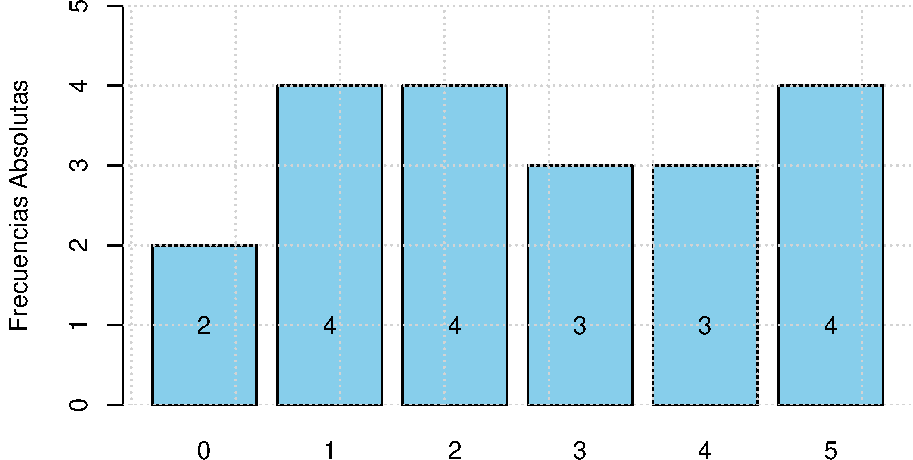
\includegraphics{BioestadisticaUnoUCES2021_files/figure-latex/unnamed-chunk-9-1.pdf}

Comando para generar la GRAFICA DE BARRAS de frecuencias relativas relacionada a la variable Pc

\begin{Shaded}
\begin{Highlighting}[]
\NormalTok{tbp <-}\StringTok{ }\KeywordTok{prop.table}\NormalTok{(}\KeywordTok{table}\NormalTok{(Pc))}
\NormalTok{barras2 <-}\StringTok{ }\KeywordTok{barplot}\NormalTok{(tbp,}\DataTypeTok{col=}\StringTok{'skyblue'}\NormalTok{, }\DataTypeTok{ylab =}\StringTok{"Frecuencias Relativas"}\NormalTok{, }\DataTypeTok{ylim=}\KeywordTok{c}\NormalTok{(}\DecValTok{0}\NormalTok{,}\FloatTok{0.25}\NormalTok{))}
\KeywordTok{text}\NormalTok{(barras2,}\KeywordTok{c}\NormalTok{(}\FloatTok{0.05}\NormalTok{,}\FloatTok{0.05}\NormalTok{),tbp}\OperatorTok{*}\DecValTok{100}\NormalTok{)}
\KeywordTok{grid}\NormalTok{()}
\end{Highlighting}
\end{Shaded}

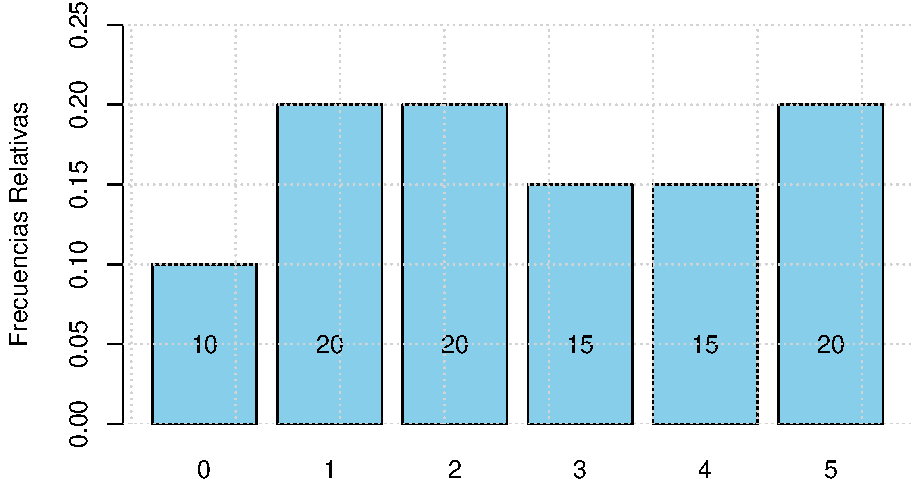
\includegraphics{BioestadisticaUnoUCES2021_files/figure-latex/unnamed-chunk-10-1.pdf}

\begin{Shaded}
\begin{Highlighting}[]
\NormalTok{Pc <-}\StringTok{ }\KeywordTok{c}\NormalTok{(}\DecValTok{5}\NormalTok{,}\DecValTok{1}\NormalTok{,}\DecValTok{3}\NormalTok{,}\DecValTok{0}\NormalTok{,}\DecValTok{2}\NormalTok{,}\DecValTok{1}\NormalTok{,}\DecValTok{5}\NormalTok{,}\DecValTok{3}\NormalTok{,}\DecValTok{2}\NormalTok{,}\DecValTok{4}\NormalTok{,}\DecValTok{1}\NormalTok{,}\DecValTok{2}\NormalTok{,}\DecValTok{4}\NormalTok{,}\DecValTok{2}\NormalTok{,}\DecValTok{0}\NormalTok{,}\DecValTok{3}\NormalTok{,}\DecValTok{5}\NormalTok{,}\DecValTok{1}\NormalTok{,}\DecValTok{5}\NormalTok{,}\DecValTok{4}\NormalTok{)}
\NormalTok{k12 <-}\KeywordTok{ncol}\NormalTok{(}\KeywordTok{matrix}\NormalTok{(Pc,}\DecValTok{1}\NormalTok{,}\DecValTok{20}\NormalTok{))}
\NormalTok{k11<-}\KeywordTok{round}\NormalTok{(}\DecValTok{1} \OperatorTok{+}\StringTok{ }\NormalTok{(}\FloatTok{3.322}\OperatorTok{*}\KeywordTok{log10}\NormalTok{(k12)),}\DataTypeTok{digits =} \DecValTok{0}\NormalTok{)}
\NormalTok{k11}
\end{Highlighting}
\end{Shaded}

\begin{verbatim}
## [1] 5
\end{verbatim}

\begin{Shaded}
\begin{Highlighting}[]
\NormalTok{Px <-}\StringTok{ }\KeywordTok{as.data.frame}\NormalTok{(}\KeywordTok{table}\NormalTok{(}\DataTypeTok{x=}\KeywordTok{factor}\NormalTok{(}\KeywordTok{cut}\NormalTok{(Pc,}\DataTypeTok{breaks=}\NormalTok{k11))))}

\NormalTok{PPx <-}\StringTok{ }\KeywordTok{transform}\NormalTok{(Px,}
               \DataTypeTok{FreAc =}\KeywordTok{cumsum}\NormalTok{(Freq),}
               \DataTypeTok{Rel=}\KeywordTok{round}\NormalTok{(}\KeywordTok{prop.table}\NormalTok{(Freq),}\DecValTok{4}\NormalTok{),}
               \DataTypeTok{RelAc=}\KeywordTok{round}\NormalTok{(}\KeywordTok{cumsum}\NormalTok{(}\KeywordTok{prop.table}\NormalTok{(Freq)),}\DecValTok{4}\NormalTok{))}
\NormalTok{knitr}\OperatorTok{::}\KeywordTok{kable}\NormalTok{(}
\NormalTok{PPx , }\DataTypeTok{caption =} \StringTok{'Tabla en Frecuencia para Datos Agrupados'}\NormalTok{,}
  \DataTypeTok{booktabs =} \OtherTok{TRUE}
\NormalTok{)}
\end{Highlighting}
\end{Shaded}

\begin{table}

\caption{\label{tab:Tabla5}Tabla en Frecuencia para Datos Agrupados}
\centering
\begin{tabular}[t]{lrrrr}
\toprule
x & Freq & FreAc & Rel & RelAc\\
\midrule
(-0.005,1] & 6 & 6 & 0.30 & 0.30\\
(1,2] & 4 & 10 & 0.20 & 0.50\\
(2,3] & 3 & 13 & 0.15 & 0.65\\
(3,4] & 3 & 16 & 0.15 & 0.80\\
(4,5] & 4 & 20 & 0.20 & 1.00\\
\bottomrule
\end{tabular}
\end{table}

Comando para obtener el histograma (ó GRAFICO) asociado a la tabla de frecuencias absolutas

\begin{Shaded}
\begin{Highlighting}[]
\NormalTok{Pc <-}\StringTok{ }\KeywordTok{c}\NormalTok{(}\DecValTok{5}\NormalTok{,}\DecValTok{1}\NormalTok{,}\DecValTok{3}\NormalTok{,}\DecValTok{0}\NormalTok{,}\DecValTok{2}\NormalTok{,}\DecValTok{1}\NormalTok{,}\DecValTok{5}\NormalTok{,}\DecValTok{3}\NormalTok{,}\DecValTok{2}\NormalTok{,}\DecValTok{4}\NormalTok{,}\DecValTok{1}\NormalTok{,}\DecValTok{2}\NormalTok{,}\DecValTok{4}\NormalTok{,}\DecValTok{2}\NormalTok{,}\DecValTok{0}\NormalTok{,}\DecValTok{3}\NormalTok{,}\DecValTok{5}\NormalTok{,}\DecValTok{1}\NormalTok{,}\DecValTok{5}\NormalTok{,}\DecValTok{4}\NormalTok{)}
\CommentTok{# table(intervalosEDAD)}
\NormalTok{tbp1 <-}\StringTok{ }\KeywordTok{table}\NormalTok{(Pc)}
\NormalTok{grahis <-}\KeywordTok{hist}\NormalTok{(Pc, }\DataTypeTok{ylab =}\StringTok{"Frecuencias Absoluta"}\NormalTok{, }\DataTypeTok{main =}\StringTok{"Histograma de clases asociados a una frecuencia absoluta "}\NormalTok{, }\DataTypeTok{col=}\StringTok{"skyblue"}\NormalTok{, }\DataTypeTok{xlab =} \StringTok{"Variable Pc"}\NormalTok{)}
\CommentTok{# text(grahis,c(1,1),tbp1)}
\KeywordTok{grid}\NormalTok{()}
\end{Highlighting}
\end{Shaded}

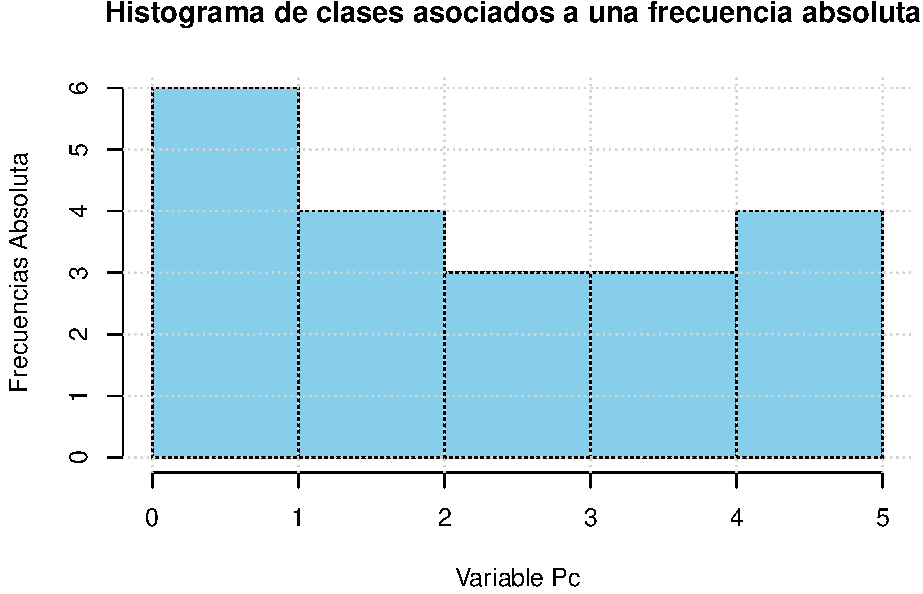
\includegraphics{BioestadisticaUnoUCES2021_files/figure-latex/unnamed-chunk-11-1.pdf}

Comando para obtener la caja de bigotes (ó GRAFICO) asociado a la variable EDAD

\hypertarget{gruxe1fica-caja-y-bigotes}{%
\subsection{Gráfica caja y bigotes}\label{gruxe1fica-caja-y-bigotes}}

\begin{Shaded}
\begin{Highlighting}[]
\KeywordTok{boxplot}\NormalTok{(Pc,}
        \DataTypeTok{main=}\StringTok{"Caja de bigotes Horizontal variable numéricas Pc"}\NormalTok{,}
        \DataTypeTok{col=}\StringTok{"skyblue"}\NormalTok{,}\DataTypeTok{horizontal=}\NormalTok{T)}
\NormalTok{values <-}\StringTok{ }\KeywordTok{c}\NormalTok{(}\KeywordTok{round}\NormalTok{(}\KeywordTok{boxplot.stats}\NormalTok{(Pc)}\OperatorTok{$}\NormalTok{conf, }\DecValTok{1}\NormalTok{), }\KeywordTok{boxplot.stats}\NormalTok{(Pc)}\OperatorTok{$}\NormalTok{stats)}
\KeywordTok{text}\NormalTok{(}\DataTypeTok{x =}\NormalTok{ values, }\DataTypeTok{labels =}\NormalTok{ values, }\DataTypeTok{y =} \FloatTok{1.25}\NormalTok{)}
\end{Highlighting}
\end{Shaded}

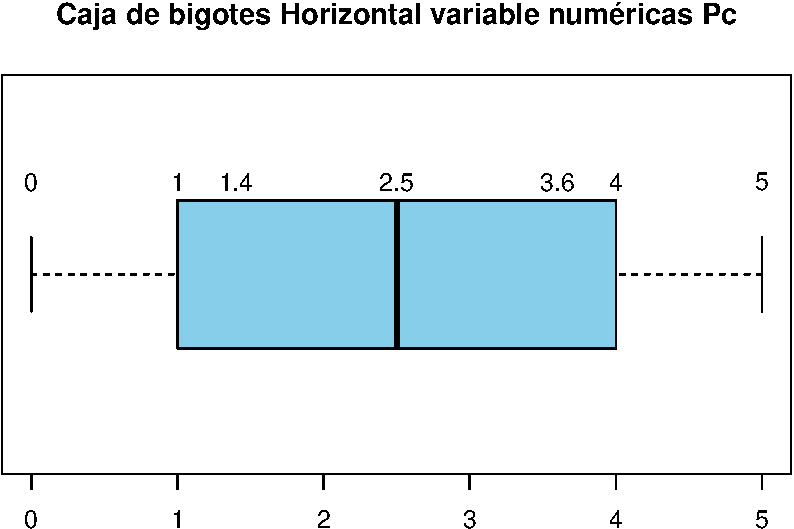
\includegraphics{BioestadisticaUnoUCES2021_files/figure-latex/unnamed-chunk-12-1.pdf}

\begin{Shaded}
\begin{Highlighting}[]
\KeywordTok{boxplot}\NormalTok{(Pc,}
        \DataTypeTok{main=}\StringTok{"Caja de bigotes Vertical variable numéricas Pc"}\NormalTok{,}
        \DataTypeTok{col=}\StringTok{"skyblue"}\NormalTok{,}\DataTypeTok{horizontal=}\NormalTok{F)}
\NormalTok{values <-}\StringTok{ }\KeywordTok{c}\NormalTok{(}\KeywordTok{round}\NormalTok{(}\KeywordTok{boxplot.stats}\NormalTok{(Pc)}\OperatorTok{$}\NormalTok{conf, }\DecValTok{1}\NormalTok{), }\KeywordTok{boxplot.stats}\NormalTok{(Pc)}\OperatorTok{$}\NormalTok{stats)}
\KeywordTok{text}\NormalTok{(}\DataTypeTok{y =}\NormalTok{ values, }\DataTypeTok{labels =}\NormalTok{ values, }\DataTypeTok{x =} \FloatTok{1.25}\NormalTok{)}
\end{Highlighting}
\end{Shaded}

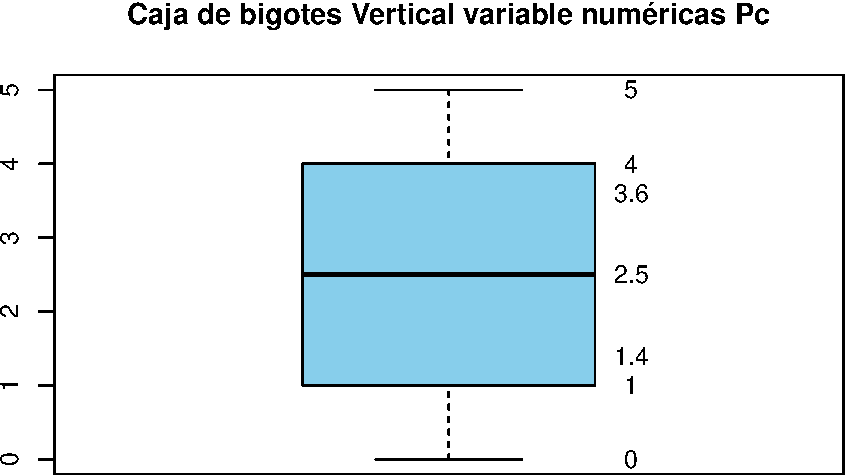
\includegraphics{BioestadisticaUnoUCES2021_files/figure-latex/unnamed-chunk-13-1.pdf}

\begin{Shaded}
\begin{Highlighting}[]
\NormalTok{Pc <-}\StringTok{ }\KeywordTok{c}\NormalTok{(}\DecValTok{5}\NormalTok{,}\DecValTok{1}\NormalTok{,}\DecValTok{3}\NormalTok{,}\DecValTok{0}\NormalTok{,}\DecValTok{2}\NormalTok{,}\DecValTok{1}\NormalTok{,}\DecValTok{5}\NormalTok{,}\DecValTok{3}\NormalTok{,}\DecValTok{2}\NormalTok{,}\DecValTok{4}\NormalTok{,}\DecValTok{1}\NormalTok{,}\DecValTok{2}\NormalTok{,}\DecValTok{4}\NormalTok{,}\DecValTok{2}\NormalTok{,}\DecValTok{0}\NormalTok{,}\DecValTok{3}\NormalTok{,}\DecValTok{5}\NormalTok{,}\DecValTok{1}\NormalTok{,}\DecValTok{5}\NormalTok{,}\DecValTok{4}\NormalTok{)}
\KeywordTok{summary}\NormalTok{(Pc)}
\end{Highlighting}
\end{Shaded}

\begin{verbatim}
##    Min. 1st Qu.  Median    Mean 3rd Qu.    Max. 
##    0.00    1.00    2.50    2.65    4.00    5.00
\end{verbatim}

\begin{itemize}
\tightlist
\item
  Ejemplo2
\end{itemize}

\textbf{Tecnología}: Se pregunto a 30 jóvenes cuántas horas didicaban cada día a navegar en internet (el tiempo que dedican a sesiones de chat y a las redes sociales quedan incluido). Los resultados son los siguientes:

\begin{equation}
\begin{matrix}
2.5 & 4.5 & 5.8 & 2.2 & 5.7\\
5.3 & 4.0 & 0.9 & 2.5 & 2.3\\
3.2 & 4.9 & 2.7 & 3.7 & 3.8\\
4.9 & 2.8 & 3.6 & 4.2 & 3.1\\
7.2 & 1.9 & 5.9 & 3.3 & 2.9\\
1.1 & 1.7 & 2.6 & 3.1 & 4.4
\end{matrix}
\end{equation}

\hypertarget{proceso-para-presentar-datos-en-forma-agrupada}{%
\section{Proceso para presentar datos en forma agrupada}\label{proceso-para-presentar-datos-en-forma-agrupada}}

\begin{itemize}
\tightlist
\item
  Obtener el tama\textasciitilde no de la muestra \((n)\).
\item
  Hallar el m'inimo y el m'aximo de los datos
\item
  Obtener el recorrido de la variable (o rango) el cual se define como:
\end{itemize}

\[
R=x_{max}-x_{min}
\]

\begin{itemize}
\tightlist
\item
  Calcular el número de intervalos (o clases) a utilizar.
\end{itemize}

Estos intervalos tambión se llaman \textbf{intervalos de clase}. La \textbf{regla de Sturges} indica que el número de intervalos de clase recomendado, es:
\[
        k=1+3,322log_{10}(n)
        \]
donde \(n\) es el tamaño de la muestra.

\begin{itemize}
\item
  Obtener la amplitud de clase. La amplitud de cada celda se calcula con la fórmula.

  \[
    a=\dfrac{R}{k}=\dfrac{x_{max}-x_{min}}{k}
    \]
\item
  Los intervalos seleccionados no pueden solaparse.
\item
  Contar el número de datos que caen en cada intervalo de clase. Dicho conteo se llama la \textbf{frecuencia absoluta} de clase.
\item
  Calcular la \textbf{frecuencia relativa de clase} dividiendo la \textbf{frecuencia absoluta de clase} por el número total de datos en la muestra.
\item
  El diagrama ubica la variable evaluada en el eje \(x\), y sobre este eje, levanta rectángulos cuyas áreas son iguales o proporcionales a la frecuencia absoluta \((n_i)\) o relativa \((f_i)\) de cada intervalo de clase.
\item
\item
  Ejemplo3
\end{itemize}

\begin{Shaded}
\begin{Highlighting}[]
\NormalTok{edad <-}\StringTok{ }\KeywordTok{c}\NormalTok{(}\DecValTok{22}\NormalTok{, }\DecValTok{34}\NormalTok{, }\DecValTok{29}\NormalTok{, }\DecValTok{25}\NormalTok{, }\DecValTok{30}\NormalTok{, }\DecValTok{33}\NormalTok{, }\DecValTok{31}\NormalTok{, }\DecValTok{27}\NormalTok{, }\DecValTok{25}\NormalTok{, }\DecValTok{25}\NormalTok{)}
\NormalTok{tiempo <-}\StringTok{ }\KeywordTok{c}\NormalTok{(}\FloatTok{14.21}\NormalTok{, }\FloatTok{10.36}\NormalTok{, }\FloatTok{11.89}\NormalTok{, }\FloatTok{13.81}\NormalTok{, }\FloatTok{12.03}\NormalTok{, }\FloatTok{10.99}\NormalTok{, }\FloatTok{12.48}\NormalTok{, }\FloatTok{13.37}\NormalTok{, }\FloatTok{12.29}\NormalTok{, }\FloatTok{11.92}\NormalTok{)}
\NormalTok{sexo <-}\StringTok{ }\KeywordTok{c}\NormalTok{(}\StringTok{"M"}\NormalTok{,}\StringTok{"H"}\NormalTok{,}\StringTok{"H"}\NormalTok{,}\StringTok{"M"}\NormalTok{,}\StringTok{"M"}\NormalTok{,}\StringTok{"H"}\NormalTok{,}\StringTok{"M"}\NormalTok{,}\StringTok{"M"}\NormalTok{,}\StringTok{"H"}\NormalTok{,}\StringTok{"H"}\NormalTok{)}
\NormalTok{misdeClase <-}\StringTok{ }\KeywordTok{data.frame}\NormalTok{(edad,tiempo,sexo)}
\KeywordTok{boxplot}\NormalTok{(misdeClase}\OperatorTok{$}\NormalTok{edad}\OperatorTok{~}\NormalTok{misdeClase}\OperatorTok{$}\NormalTok{sexo,}\DataTypeTok{horizontal =}\NormalTok{ T)}
\NormalTok{Pc <-}\StringTok{ }\NormalTok{misdeClase}\OperatorTok{$}\NormalTok{edad}
\NormalTok{values <-}\StringTok{ }\KeywordTok{c}\NormalTok{(}\KeywordTok{round}\NormalTok{(}\KeywordTok{boxplot.stats}\NormalTok{(Pc)}\OperatorTok{$}\NormalTok{conf, }\DecValTok{1}\NormalTok{), }\KeywordTok{boxplot.stats}\NormalTok{(Pc)}\OperatorTok{$}\NormalTok{stats)}
\KeywordTok{text}\NormalTok{(}\DataTypeTok{x =}\NormalTok{ values, }\DataTypeTok{labels =}\NormalTok{ values, }\DataTypeTok{y =} \FloatTok{1.5}\NormalTok{)}
\end{Highlighting}
\end{Shaded}

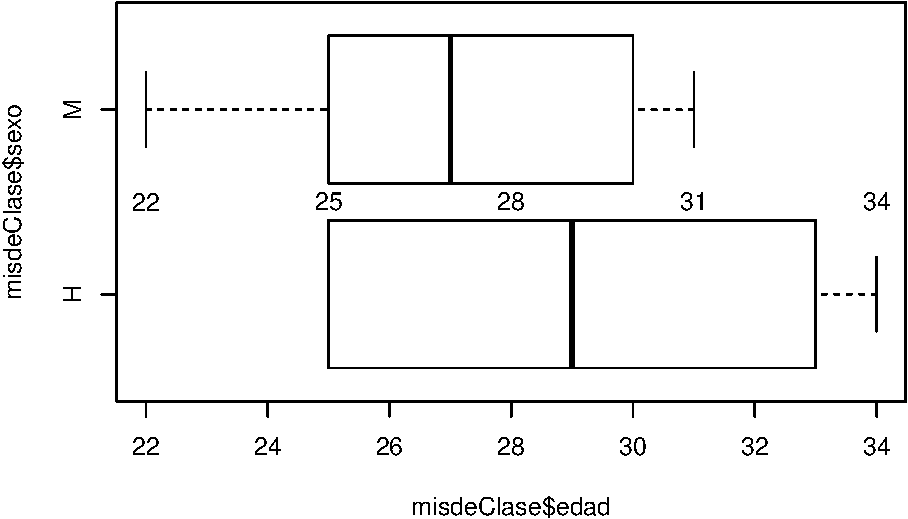
\includegraphics{BioestadisticaUnoUCES2021_files/figure-latex/unnamed-chunk-15-1.pdf}

\begin{Shaded}
\begin{Highlighting}[]
\NormalTok{edad <-}\StringTok{ }\KeywordTok{c}\NormalTok{(}\DecValTok{22}\NormalTok{, }\DecValTok{34}\NormalTok{, }\DecValTok{29}\NormalTok{, }\DecValTok{25}\NormalTok{, }\DecValTok{30}\NormalTok{, }\DecValTok{33}\NormalTok{, }\DecValTok{31}\NormalTok{, }\DecValTok{27}\NormalTok{, }\DecValTok{25}\NormalTok{, }\DecValTok{25}\NormalTok{)}
\NormalTok{tiempo <-}\StringTok{ }\KeywordTok{c}\NormalTok{(}\FloatTok{14.21}\NormalTok{, }\FloatTok{10.36}\NormalTok{, }\FloatTok{11.89}\NormalTok{, }\FloatTok{13.81}\NormalTok{, }\FloatTok{12.03}\NormalTok{, }\FloatTok{10.99}\NormalTok{, }\FloatTok{12.48}\NormalTok{, }\FloatTok{13.37}\NormalTok{, }\FloatTok{12.29}\NormalTok{, }\FloatTok{11.92}\NormalTok{)}
\NormalTok{sexo <-}\StringTok{ }\KeywordTok{c}\NormalTok{(}\StringTok{"M"}\NormalTok{,}\StringTok{"H"}\NormalTok{,}\StringTok{"H"}\NormalTok{,}\StringTok{"M"}\NormalTok{,}\StringTok{"M"}\NormalTok{,}\StringTok{"H"}\NormalTok{,}\StringTok{"M"}\NormalTok{,}\StringTok{"M"}\NormalTok{,}\StringTok{"H"}\NormalTok{,}\StringTok{"H"}\NormalTok{)}
\NormalTok{misdeClase <-}\StringTok{ }\KeywordTok{data.frame}\NormalTok{(edad,tiempo,sexo)}
\KeywordTok{boxplot}\NormalTok{(misdeClase}\OperatorTok{$}\NormalTok{tiempo}\OperatorTok{~}\NormalTok{misdeClase}\OperatorTok{$}\NormalTok{sexo,}\DataTypeTok{horizontal =}\NormalTok{ T)}
\NormalTok{P1c <-}\StringTok{ }\NormalTok{misdeClase}\OperatorTok{$}\NormalTok{tiempo}
\NormalTok{values <-}\StringTok{ }\KeywordTok{c}\NormalTok{(}\KeywordTok{round}\NormalTok{(}\KeywordTok{boxplot.stats}\NormalTok{(P1c)}\OperatorTok{$}\NormalTok{conf, }\DecValTok{1}\NormalTok{), }\KeywordTok{boxplot.stats}\NormalTok{(P1c)}\OperatorTok{$}\NormalTok{stats)}
\KeywordTok{text}\NormalTok{(}\DataTypeTok{x =}\NormalTok{ values, }\DataTypeTok{labels =}\NormalTok{ values, }\DataTypeTok{y =} \FloatTok{1.5}\NormalTok{)}
\end{Highlighting}
\end{Shaded}

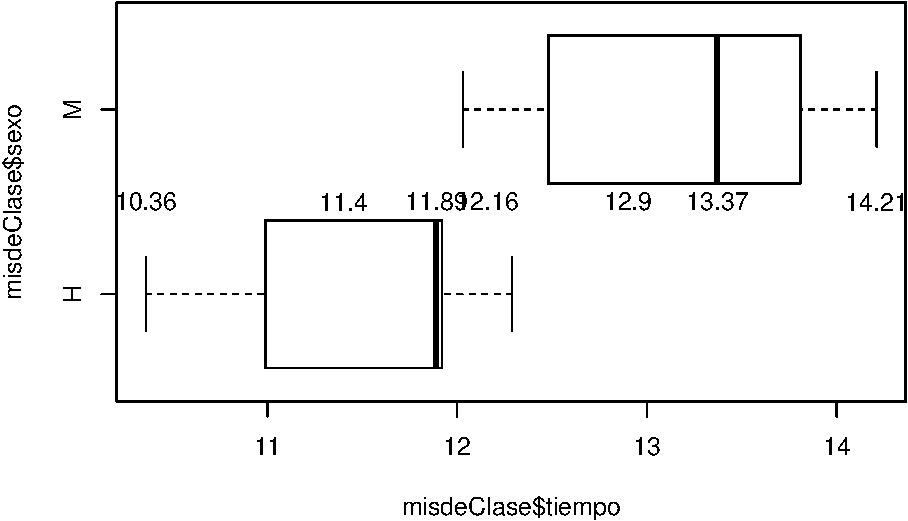
\includegraphics{BioestadisticaUnoUCES2021_files/figure-latex/unnamed-chunk-16-1.pdf}

\begin{Shaded}
\begin{Highlighting}[]
\NormalTok{edad <-}\StringTok{ }\KeywordTok{c}\NormalTok{(}\DecValTok{22}\NormalTok{, }\DecValTok{34}\NormalTok{, }\DecValTok{29}\NormalTok{, }\DecValTok{25}\NormalTok{, }\DecValTok{30}\NormalTok{, }\DecValTok{33}\NormalTok{, }\DecValTok{31}\NormalTok{, }\DecValTok{27}\NormalTok{, }\DecValTok{25}\NormalTok{, }\DecValTok{25}\NormalTok{)}
\NormalTok{tiempo <-}\StringTok{ }\KeywordTok{c}\NormalTok{(}\FloatTok{14.21}\NormalTok{, }\FloatTok{10.36}\NormalTok{, }\FloatTok{11.89}\NormalTok{, }\FloatTok{13.81}\NormalTok{, }\FloatTok{12.03}\NormalTok{, }\FloatTok{10.99}\NormalTok{, }\FloatTok{12.48}\NormalTok{, }\FloatTok{13.37}\NormalTok{, }\FloatTok{12.29}\NormalTok{, }\FloatTok{11.92}\NormalTok{)}
\NormalTok{sexo <-}\StringTok{ }\KeywordTok{c}\NormalTok{(}\StringTok{"M"}\NormalTok{,}\StringTok{"H"}\NormalTok{,}\StringTok{"H"}\NormalTok{,}\StringTok{"M"}\NormalTok{,}\StringTok{"M"}\NormalTok{,}\StringTok{"H"}\NormalTok{,}\StringTok{"M"}\NormalTok{,}\StringTok{"M"}\NormalTok{,}\StringTok{"H"}\NormalTok{,}\StringTok{"H"}\NormalTok{)}
\NormalTok{misdeClase <-}\StringTok{ }\KeywordTok{data.frame}\NormalTok{(edad,tiempo,sexo)}
\KeywordTok{boxplot}\NormalTok{(misdeClase}\OperatorTok{$}\NormalTok{tiempo}\OperatorTok{~}\NormalTok{misdeClase}\OperatorTok{$}\NormalTok{sexo,}\DataTypeTok{horizontal =}\NormalTok{ F)}
\NormalTok{P1c <-}\StringTok{ }\NormalTok{misdeClase}\OperatorTok{$}\NormalTok{tiempo}
\NormalTok{values <-}\StringTok{ }\KeywordTok{c}\NormalTok{(}\KeywordTok{round}\NormalTok{(}\KeywordTok{boxplot.stats}\NormalTok{(P1c)}\OperatorTok{$}\NormalTok{conf, }\DecValTok{1}\NormalTok{), }\KeywordTok{boxplot.stats}\NormalTok{(P1c)}\OperatorTok{$}\NormalTok{stats)}
\KeywordTok{text}\NormalTok{(}\DataTypeTok{y =}\NormalTok{ values, }\DataTypeTok{labels =}\NormalTok{ values, }\DataTypeTok{x =} \FloatTok{1.5}\NormalTok{)}
\end{Highlighting}
\end{Shaded}

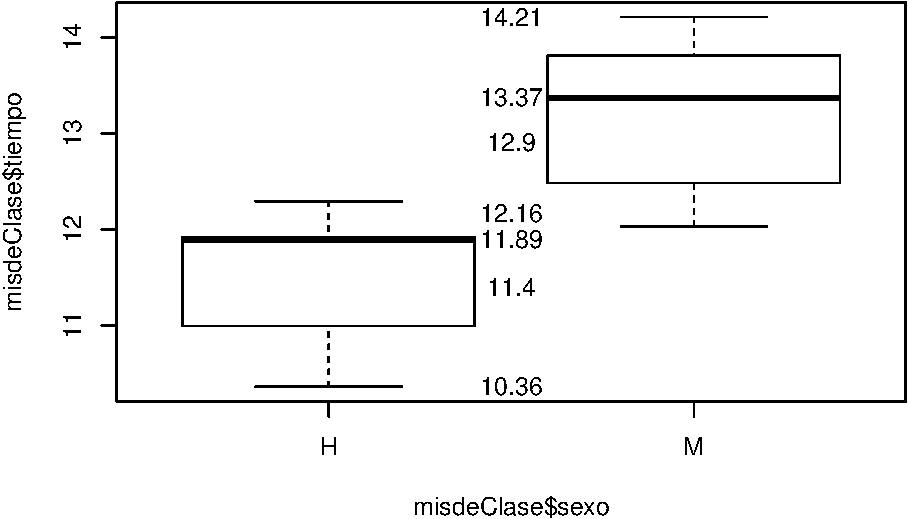
\includegraphics{BioestadisticaUnoUCES2021_files/figure-latex/unnamed-chunk-17-1.pdf}

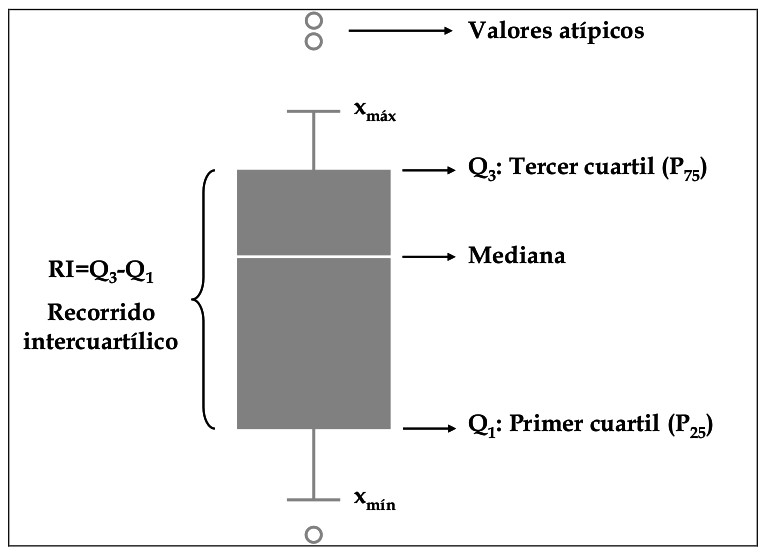
\includegraphics[width=0.55\textwidth,height=\textheight]{/home/john/Documentos/MatematicasBioEstadisticaV1/BioestadisticaUnoUCES2021/images/GRAFICAdatosAGRUPADOS8.jpg}

\hypertarget{cruxedterio-datos-atuxedpicos}{%
\subsection{\texorpdfstring{Críterio datos \textbf{atípicos}}{Críterio datos atípicos}}\label{cruxedterio-datos-atuxedpicos}}

\[
\text{Dato atípico}>Q_{3}+1.5(Q_{3}-Q_{1})
\]
\[
\text{Dato atípico}<Q_{1}-1.5(Q_{3}-Q_{1})
\]

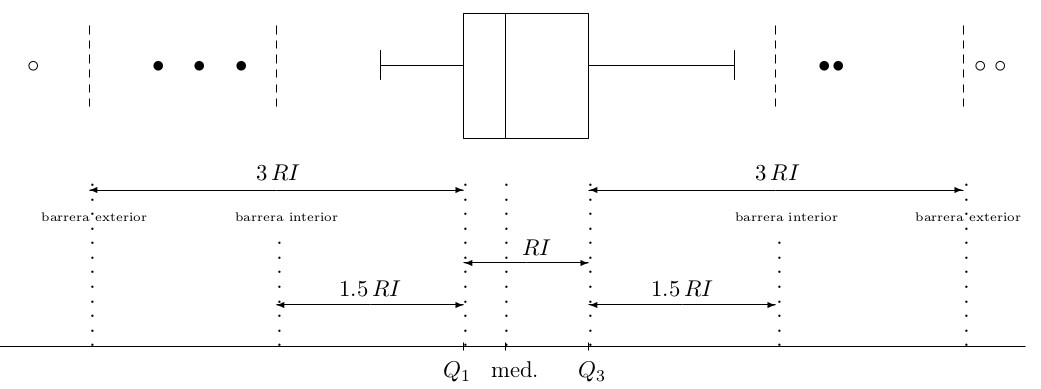
\includegraphics[width=0.85\textwidth,height=\textheight]{/home/john/Documentos/MatematicasBioEstadisticaV1/BioestadisticaUnoUCES2021/images/GRAFICAcajaybigotes12.jpg}

\hypertarget{datos-no-agrupados}{%
\section{Datos no agrupados}\label{datos-no-agrupados}}

Las siguientes son recomendaciones en el tratamiento de datos no agrupados.

\begin{itemize}
\tightlist
\item
  Ordenar los datos de menor a mayor.
\item
  Colocar una etiqueta numérica para tener clara la posición que tiene el datos en el ordenamiento.
\end{itemize}

\hypertarget{medidas-de-posiciuxf3n}{%
\subsection{Medidas de posición}\label{medidas-de-posiciuxf3n}}

Todas ellas a su manera tratan de dar una idea del número alrededor del cual se centra a todo el conjunto de datos.

\hypertarget{la-media-aritmuxe9tica-para-datos-no-agrupados-barx}{%
\subsection{\texorpdfstring{La media aritmética para datos no agrupados \((\bar{x})\)}{La media aritmética para datos no agrupados (\textbackslash bar\{x\})}}\label{la-media-aritmuxe9tica-para-datos-no-agrupados-barx}}

\[
        \bar{x}=\dfrac{\sum^{n}_{i=1}x_{i}}{n}
\]

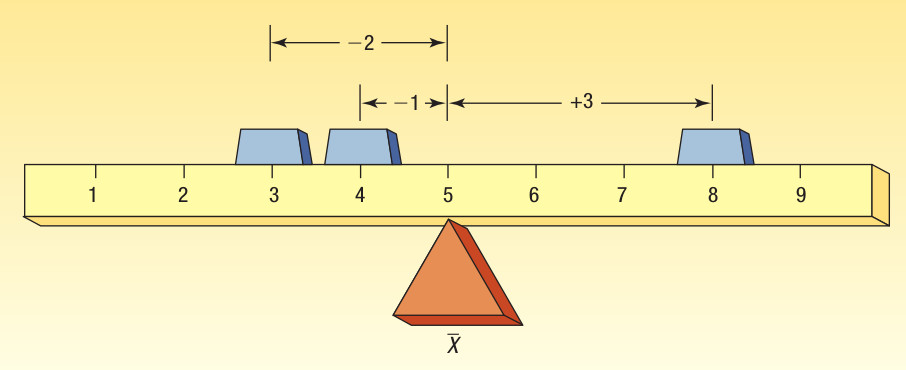
\includegraphics[width=0.55\textwidth,height=\textheight]{/home/john/Documentos/MatematicasBioEstadisticaV1/BioestadisticaUnoUCES2021/images/GRAFICAlamedia12.jpg}

\hypertarget{la-mediana-para-datos-no-agrupados}{%
\subsection{La mediana para datos no agrupados}\label{la-mediana-para-datos-no-agrupados}}

El número \(n\) es impar

\[Me=X_{\frac{n+1}{2}}\]
El número \(n\) es par

\[Me=\dfrac{X_{\frac{n}{2}}+X_{\frac{n+2}{2}}}{2}\]

\hypertarget{la-moda-m_0}{%
\subsection{\texorpdfstring{La Moda \((M_{0})\)}{La Moda (M\_\{0\})}}\label{la-moda-m_0}}

Es la medida de posición que indica la magnitud del valor que se presenta con más frecuencia en una serie de datos.

\hypertarget{cuxe1lculo-de-cuartiles-en-datos-no-agrupados}{%
\subsection{Cálculo de cuartiles en datos NO agrupados}\label{cuxe1lculo-de-cuartiles-en-datos-no-agrupados}}

Sea el conjunto de datos no agrupados:

\[
    20,23,24,24,24,25,29,31,31,33,34,36,36,37,39,39,40,40,41,45
\]
* Proceso \(Q_{1}:\)
El primer cuartil es el valor mayor que el \(25 \%\) de los valores de la distribuci'on. como N=20 resulta que

\[
\dfrac{n}{4}=5
\]
el primer cuartil es la media aritm'etica de dicho valor y el siguiente:

\[
Q_{1}=\dfrac{24+25}{2}=24.5
\]
Sea el conjunto de datos no agrupados:

\[
    20,23,24,24,24,25,29,31,31,33,34,36,36,37,39,39,40,40,41,45
\]

\begin{itemize}
\tightlist
\item
  Proceso \(Q_{2}:\)
\end{itemize}

El segundo cuartil es, evidentemente, la medianan de la distribución, es el valor de la variable que ocupa el lugar central en un conjunto de datos ordenados. Ccomo N=20 resulta que

\[
\dfrac{n}{2}=10
\]

la mediana es la media aritm'etica de dicho valor y el siguiente:

\[
M_{e}=Q_{2}=\dfrac{33+34}{2}=33.5
\]
Sea el conjunto de datos no agrupados:

\[
    20,23,24,24,24,25,29,31,31,33,34,36,36,37,39,39,40,40,41,45
\]

\begin{itemize}
\tightlist
\item
  Proceso \(Q_{3}:\)
\end{itemize}

El tercer cuartil es, el valor que sobrepasa al \(75 \%\) de los valores de la distribución. En nuestro caso, como \(N=20\) resulta que

\[
\dfrac{3n}{4}=15
\]

resulta:

\[
Q_{3}=\dfrac{39+39}{2}=39
\]

\hypertarget{datos-agrupados}{%
\section{Datos agrupados}\label{datos-agrupados}}

Dada la siguiente distribución correspondiente al salario samanal en dòlares para un grupo de obreros en una empresa petrolera tradicional

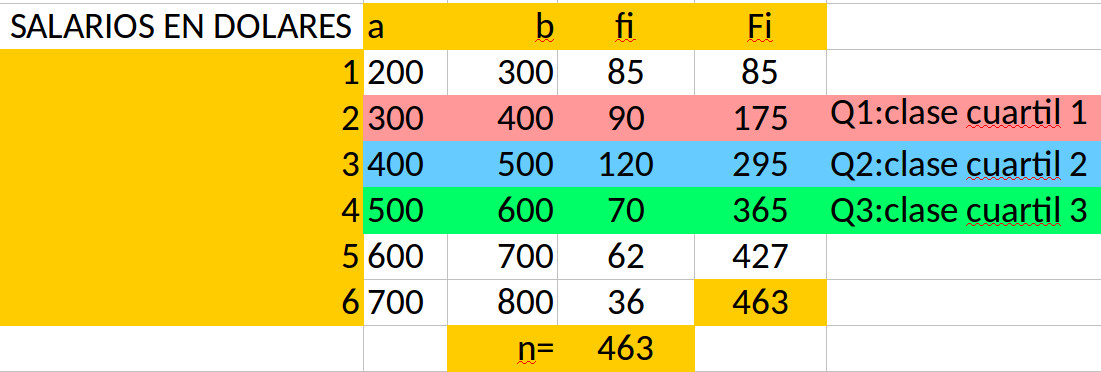
\includegraphics[width=0.75\textwidth,height=\textheight]{/home/john/Documentos/MatematicasBioEstadisticaV1/BioestadisticaUnoUCES2021/images/GRAFICAdatosAGRUPADOS7.jpg}

Obtener:

\begin{itemize}
\item
  La media \((\bar{x}=?)\)
\item
  La mediana \((Me=?)\)
\item
  La moda \((Mo=?)\)
\item
  El primer cuartil \((Q_1=?)\)
\item
  El segundo cuartil \((Q_2=?)\)
\item
  El tercer cuartil \((Q_3=?)\)
\item
  La varianza \((\sigma^2=?)\)
\item
  La desviación estándar \((\sqrt{\sigma^2}=\sigma=?)\)
\end{itemize}

En la distribución de frecuencias correspondiente al peso en \(Kg\) para un grupo de obreros.

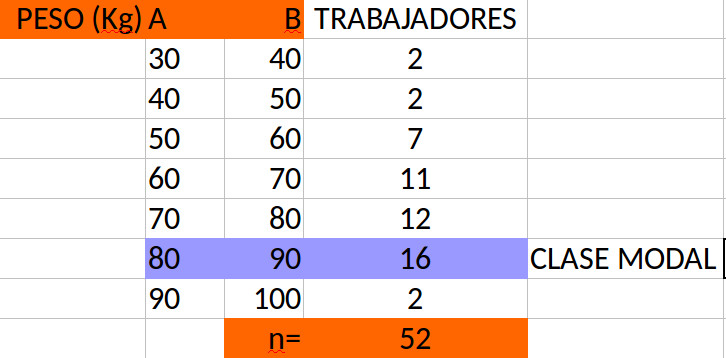
\includegraphics[width=0.65\textwidth,height=\textheight]{/home/john/Documentos/MatematicasBioEstadisticaV1/BioestadisticaUnoUCES2021/images/GRAFICAdatosAGRUPADOS5.jpg}

Calcule:

\begin{itemize}
\item
  La media \((\bar{x}=?)\)
\item
  La mediana \((Me=?)\)
\item
  La moda \((Mo=?)\)
\item
  El primer cuartil \((Q_1=?)\)
\item
  El segundo cuartil \((Q_2=?)\)
\item
  El tercer cuartil \((Q_3=?)\)
\item
  La varianza \((\sigma^2=?)\)
\item
  La desviación estándar \((\sqrt{\sigma^2}=\sigma=?)\)
\end{itemize}

Para la tabla de distribución en frecuencias correspondiente a las horas extras laboradas por un grupo de obreros

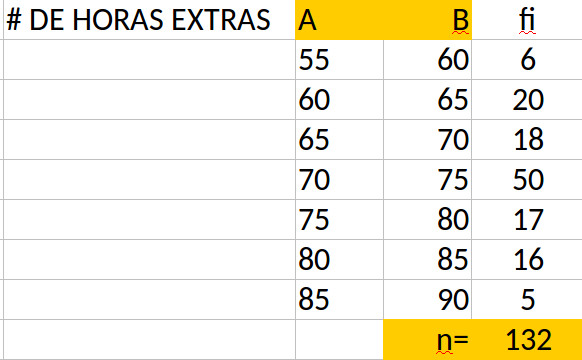
\includegraphics[width=0.55\textwidth,height=\textheight]{/home/john/Documentos/MatematicasBioEstadisticaV1/BioestadisticaUnoUCES2021/images/GRAFICAdatosAGRUPADOS3.jpg}

Realice el cálculo de:

\begin{itemize}
\item
  La media \((\bar{x}=?)\)
\item
  La mediana \((Me=?)\)
\item
  La moda \((Mo=?)\)
\item
  El primer cuartil \((Q_1=?)\)
\item
  El segundo cuartil \((Q_2=?)\)
\item
  El tercer cuartil \((Q_3=?)\)
\item
  La varianza \((\sigma^2=?)\)
\item
  La desviación estándar \((\sqrt{\sigma^2}=\sigma=?)\)
\end{itemize}

\begin{figure}

{\centering 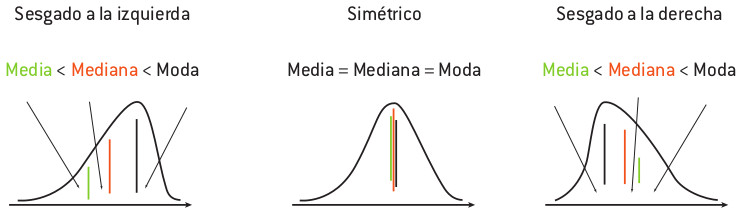
\includegraphics[width=10.42in]{/home/john/Documentos/MatematicasBioEstadisticaV1/BioestadisticaUnoUCES2021/images/Sesgo1} 

}

\caption{Medidas de tendencia central y de dispersión [Imagen tomada de [@gutierrez2012probabilidad] pág $51$]}\label{fig:Sesgo1}
\end{figure}

\begin{itemize}
\item
  \textbf{Simétrica}, si la mayor concentración de datos se localiza en el centro de la distribución
\item
  \textbf{Sesgada a derecha}, si la mayor concentración de datos se localiza a la izquierda de la distribución
\item
  \textbf{Sesgada a izquierda}, si la mayor concentración de datos se localiza a la derecha de la distribución
\end{itemize}

\hypertarget{la-media-para-datos-agrupados-barx}{%
\subsection{\texorpdfstring{La media para datos agrupados \((\bar{x})\)}{La media para datos agrupados (\textbackslash bar\{x\})}}\label{la-media-para-datos-agrupados-barx}}

\[
\bar{x}=\dfrac{\sum_{i=1}^{n}f_{i}x_{i}}{n}
\]

\hypertarget{la-mediana-para-datos-agrupados-me}{%
\subsection{\texorpdfstring{La mediana para datos agrupados \((Me)\)}{La mediana para datos agrupados (Me)}}\label{la-mediana-para-datos-agrupados-me}}

Proceso:

\begin{itemize}
\item
  Se elabora la tabla de frecuencias de datos con diferentes intervalos de clases, se ubican las frecuencias absolutas \(n_{i}\) y se calculan las frecuencias acumuladas \(F_{i}\) de la distribución.
\item
  Se determina la ubicación o posición de la mediana en el intervalo de la distribución de frecuencia, mediante la fórmula \(\frac{n}{2}\). Esta clase se llamará clase de la mediana. El resultado obtenido determinarí la clase donde se encuentra ubicada \(f_{i}\) sea igual o superior a este resultado. Luego se aplica la fórmula:
\end{itemize}

\[Me=L_{i}+\left( \dfrac{\frac{n}{2}-F_{i-1}}{f_{i}}\right) I_c\]

\begin{itemize}
\tightlist
\item
  \(\frac{n}{2}\): Posición de la mediana.\textbf{()}
\end{itemize}

Este valor de posición se comparó con las datos que se tienen en la columna (\textbf{\(F_i\)}), y posteriormente se selecciona el valor más proximo pero mayor que \(\frac{n}{2}\). El intervalo donde se encontro dicho valor se denomina ``\textbf{Intervalo de la mediana}''

\begin{itemize}
\item
  \(L_{i}\): Es el limite inferior de la clase donde se ubicada la mediana.
\item
  \(F_{(i-1)}\): Es el valor de la frecuencia acumulada anterior a la clase mediana.
\item
  \(f_{i}\): Es el valor de la frecuencia de clase donde se encuentra la mediana.
\item
  \(I_{c}\): Es el tamaño del intervalo de clase.
\item
  \(n\): Es el número total de datos de la distribuación en estudio.
\end{itemize}

\hypertarget{los-cuartiles-para-datos-agrupados-q_c}{%
\subsection{\texorpdfstring{Los cuartiles para datos agrupados \((Q_c)\)}{Los cuartiles para datos agrupados (Q\_c)}}\label{los-cuartiles-para-datos-agrupados-q_c}}

\[Q_c=L_{i}+\left( \dfrac{\frac{cn}{4}-F_{(i-1)}}{f_{i}}\right) I_c\]

Se inicia determinando la posición que ocupa el cuartil solicitado mediante la fórmula

Posición de clase para el cuartil \(c\);

\[
P_{c}=\dfrac{cn}{4}
\]
\(\frac{cn}{4}\): Posición que ocupa el cuartil en la distribución de frecuencia.

Este valor de posición se comparó con las datos que se tienen en la columna (\textbf{\(F_i\)}), y posteriormente se selecciona el valor más proximo pero mayor que \(\frac{n}{2}\). El intervalo donde se encontro dicho valor se denomina ``\textbf{Intervalo intercuartílico \(Q_c\)}''

\(c\): Corresponde al número del cuartil solicitado: \(1,2,3\).

\(L_{i}\): Es el limite inferior de la clase donde se encuentra ubicado el cuartil deseado.

\hypertarget{la-moda-para-datos-agrupados-mo}{%
\subsection{\texorpdfstring{La moda para datos agrupados \((Mo)\)}{La moda para datos agrupados (Mo)}}\label{la-moda-para-datos-agrupados-mo}}

\[
M_{o}=L_{i}+\left( \dfrac{\vartriangle_{1}}{\vartriangle_{1}+\vartriangle_{2}}\right) I_c
\]

\(L_{i}\): Es el limite inferior de la clase modal.

\(\vartriangle_{1}\):Es la diferencia entre la frecuencia absoluta de la clase modal y la frecuencia de la clase anterior a la modal.

\(\vartriangle_{2}\):Es la diferencia entre la frecuencia absoluta de la clase modal y la frecuencia de la clase siguiente a la modal.

\(I_{c}\): Es el tamaño del intervalo de clase.

\hypertarget{cuxe1lculo-de-deciles-para-datos-agrupados.}{%
\subsection{Cálculo de Deciles para datos agrupados.}\label{cuxe1lculo-de-deciles-para-datos-agrupados.}}

\[
D_k=L_{i}+\left( \dfrac{\frac{kn}{10}-F_{(i-1)}}{f_{i}}\right) I_c
\]

\hypertarget{percentil-para-datos-agrupados.}{%
\subsection{Percentil para datos agrupados.}\label{percentil-para-datos-agrupados.}}

\[
P_k=L_{i}+\left( \dfrac{\frac{kn}{100}-F_{(i-1)}}{f_{i}}\right) I_c
\]

\begin{figure}

{\centering 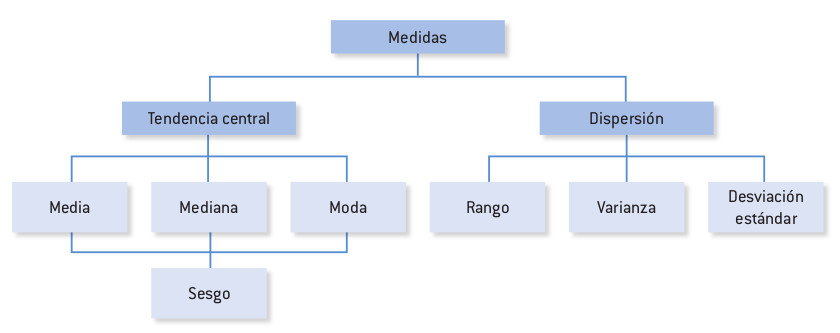
\includegraphics[width=11.67in]{/home/john/Documentos/MatematicasBioEstadisticaV1/BioestadisticaUnoUCES2021/images/MedidasDeTendenciaCentralYDispersion1} 

}

\caption{Medidas de tendencia central y de dispersión [Imagen tomada de [@gutierrez2012probabilidad] pág $46$]}\label{fig:Estadistica2}
\end{figure}

\hypertarget{medidas-de-dispersiuxf3n}{%
\section{Medidas de dispersión}\label{medidas-de-dispersiuxf3n}}

La medida de dispersión es un número que nos indica el grado de separación en un conjunto de datos. Si el valor de la dispersión es pequeño (respecto de la unidad de medida)
entonces hay una gran uniformidad entre los datos (homogénea)

Por el contrario, un gran valor en la dispersión nos indica poca uniformidad
(heterogénea). Cuando es cero quiere decir que todos los datos son iguales. Las medidas
de dispersión se clasifican en dos grupos

\begin{itemize}
\tightlist
\item
  \textbf{Dispersión absoluta}
\end{itemize}

Entre ellas el rango, el rango intercuartilico, la desviación media, la varianza y la desviación típica.

\[
\text{Para datos no agrupados}: \ \text{DM}=\dfrac{\sum\left| x_{i}-\bar{x} \right| }{n}=\dfrac{\sum\left| d_{i} \right|}{n} 
\]
\[
\text{Para datos agrupados}: \ \text{DM}=\dfrac{\sum\left| x_{PM}-\bar{x} \right|f_{i} }{n}=\dfrac{\sum x_{i}\left| d_{i} \right|}{n} 
\]

\begin{itemize}
\tightlist
\item
  \textbf{Dispersión relativa}
\end{itemize}

La que tiene mayor importancia es el coeficiente de variación.

El valor numérico de la varianza es mayor cuando más dispersión tienen los valores de la
variable en estudio, y por tanto, cuanto menos representativa es la media.

El coeficiente de variación (ó coeficiente de Pearson) \(CV\), se define por el cociente
entre la desviación típica (ó estándar) y la media aritmética de la variable e indica,
por tanto, el número de veces que la desviación típica contiene a la media.

\[
CV=\dfrac{S}{\bar{x}}\times 100 \%
\]
El inconveniente de esta medida es que si es igual a cero el denominador de la fracción;
es decir, la media de la variable, carece de significado.

El valor mínimo del coeficiente de variación es cero, que es el valor que toma cuando es
igual a cero el numerador de la fracción; es decir, la variación típica. En tal caso,
todos los valores de la variable son iguales a la media, de manera que la dispersión de
los valores en torno a la media es nula y la media es la representación perfecta de la
serie de datos.

La media es tanto más representativa cuando más próximo a cero está el coeficiente de
variación , y cuanto más elevado es el coeficiente de variación, menos representativa es
la media.

\textbf{NOTA:}

La varianza es más significativa cuando se comparan dos o más conjuntos de
observaciones.

\begin{itemize}
\tightlist
\item
  \textbf{Varianza para datos no agrupados}
\end{itemize}

\[
S^{2}=\dfrac{\sum ( x_{i}-\bar{x})^{2}}{n}
\]

\begin{itemize}
\tightlist
\item
  \textbf{Varianza para datos agrupados}
\end{itemize}

\[
S^{2}=\dfrac{\sum n_{i}( x_{i}-\bar{x})^{2}}{n-1}
\]

\begin{itemize}
\tightlist
\item
  \textbf{Desviación típica para datos no agrupados}
\end{itemize}

\[
S=\sqrt{\dfrac{\sum ( x_{i}-\bar{x})^{2}}{n}}
\]

\begin{itemize}
\tightlist
\item
  \textbf{Desviación típica para datos agrupados}
\end{itemize}

\[
S=\sqrt{\dfrac{\sum n_{i}( x_{i}-\bar{x})^{2}}{n-1}}
\]

\hypertarget{coeficiente-para-variaciuxf3n-de-karl-pearson}{%
\section{Coeficiente para variación de Karl Pearson}\label{coeficiente-para-variaciuxf3n-de-karl-pearson}}

Este es un criterio numérico para determinar la simetría (ó sesgo) en un histograma o en
una gráfica poligonal continua

\[
A_{p}=\dfrac{\bar{x}-M_{0}}{S}
\]

\begin{itemize}
\item
  Asimétria por la derecha (ó distribuación es asimétrica positiva) \((M_{0}<\bar{x})\), y \(A_{p}>0\)
\item
  Asimétria por la izquierda (ó distribución es asimétrica negativa) \((\bar{x}<M_{0})\) y \(A_{p}<0\)
\item
  Asimétria \(A_{p}=0\)
\end{itemize}

\hypertarget{probabilidad}{%
\chapter{Probabilidad}\label{probabilidad}}

\hypertarget{teoruxeda-de-conjuntos}{%
\section{Teoría de conjuntos}\label{teoruxeda-de-conjuntos}}

\begin{definition}
\protect\hypertarget{def:unnamed-chunk-19}{}{\label{def:unnamed-chunk-19} }Un \textbf{conjunto} es una colección bien definida de objetos, llamados sus elementos. Los conjuntos se simbolizan con letras minúsculas \(A\), \(B\), \(...\) Los objetos que componen el conjunto se denominan elementos y se denotan con letras minúsculas \(a, b, ...\) {[}Tomado de \citep{zill2012algebra} pág \(21\){]}
\end{definition}

\begin{definition}
\protect\hypertarget{def:unnamed-chunk-20}{}{\label{def:unnamed-chunk-20} }Para definir un \textbf{conjunto por extensión}, se enumeran todos sus elementos separándolos por comas y luego se encierran entre llaves.

Para escribir un \textbf{conjunto por comprensión} se elige un elemento arbitrario \(x\) y se señala que cumple la propiedad \(P(x)\). Finalmente, se encierra toda la expresión entre llaves. {[}Tomado de \citep{zill2012algebra} pág \(22\){]}
\end{definition}

\[
A=\{ x | x \ \ \text{cumple la propiedad} \ \ P(x)   \}
\]

\begin{definition}
\protect\hypertarget{def:unnamed-chunk-21}{}{\label{def:unnamed-chunk-21} }Diremos que dos conjutnos \(A\) y \(B\) son iguales si tienen los mismos elementos. Para indicar que \(A\) y \(B\) son iguales se escribe:{[}Tomado de \citep{zill2012algebra} pág \(22\){]}
\end{definition}

\[
A=B
\]

\begin{remark}
\iffalse{} {Nota:} \fi{}Un conjunto que posee un número finito de elementos; se llaman \textbf{conjuntos finitos}.

Un conjunto que no tiene un número finito de elemenos se llaman \textbf{conjunto infinito}.

{[}Tomado de \citep{zill2012algebra} pág \(23\){]}
\end{remark}

\begin{definition}
\protect\hypertarget{def:unnamed-chunk-23}{}{\label{def:unnamed-chunk-23} }El número de elementos de un conjunto finito es lo que se llama la \textbf{cardinalidad} de dicho conjunto. La cardinalidad de un conjunto finito \(A\) se denota por: {[}Tomado de \citep{zill2012algebra} pág \(24\){]}
\end{definition}

\[
Card(A) \ \ \ \text{ó}  \ \ \ |A|
\]

\begin{definition}
\protect\hypertarget{def:unnamed-chunk-24}{}{\label{def:unnamed-chunk-24} }Dos conjuntos finitos \(X\) y \(Y\) se dicen ser \textbf{equipotentes} si tienen exactamente el mismo número de elementos. {[}Tomado de \citep{zill2012algebra} pág \(24\){]}
\end{definition}

\begin{definition}
\protect\hypertarget{def:unnamed-chunk-25}{}{\label{def:unnamed-chunk-25} }Un conjunto se dice \textbf{vacío} si no posee elementos. El conjunto vacío se denota como:
\end{definition}

\[
\{ \} \ \ \ \text{ó}  \ \ \ \Phi
\]

\begin{definition}
\protect\hypertarget{def:unnamed-chunk-26}{}{\label{def:unnamed-chunk-26} }El conjunto \textbf{universal} se define como el conjunto que posee todos los elementos de todos los conjuntos, y se denota como:{[}Tomado de \citep{zill2012algebra} pág \(25\){]}
\end{definition}

\[
\text{Conjunto universal:} \ \ \ U
\]

\begin{definition}
\protect\hypertarget{def:unnamed-chunk-27}{}{\label{def:unnamed-chunk-27} }Si cada elemento de un conjunto \(A\) es también elemento de un conjunto \(B\), entonces se dice que \(A\) es un subconjunto de \(B\). Se dice también que \(A\) está contenido en \(B\) o que \(B\) contiene a \(A\). La relación de subconjunto se denota como: {[}Tomado de \citep{zill2012algebra} pág \(25\){]}
\end{definition}

\[
A \subset B  \ \ \ \text{ó}  \ \ \ B \supset A
\]

\begin{figure}

{\centering 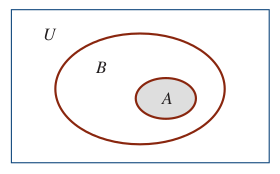
\includegraphics[width=0.6\linewidth]{/home/john/Documentos/MatematicasBioEstadisticaV1/BioestadisticaUnoUCES2021/images/Figconjunto1} 

}

\caption{Relación de subconjunto [Imagen tomada de [@zill2012algebra] pág $26$]}\label{fig:Figconjunto1}
\end{figure}

\begin{definition}
\protect\hypertarget{def:unnamed-chunk-28}{}{\label{def:unnamed-chunk-28} }La unión de dos conjuntos \(A\) y \(B\) consta de todos los elementos que pertenecen a \(A\) o a \(B\). La unión de \(A\) y \(B\) se denota por \(A \cup B\). {[}Tomado de \citep{zill2012algebra} pág \(31\){]}
\end{definition}

\[
A \cup B = \{ x | x \in A \ \text{o} \ x \in B\}
\]

\begin{figure}

{\centering 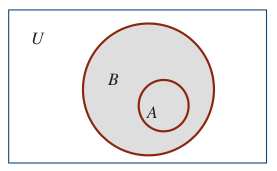
\includegraphics[width=0.6\linewidth]{/home/john/Documentos/MatematicasBioEstadisticaV1/BioestadisticaUnoUCES2021/images/FigUniona1} 

}

\caption{Relación de subconjunto [Imagen tomada de [@zill2012algebra] pág $32$]}\label{fig:FigUnionA-1}
\end{figure}
\begin{figure}

{\centering 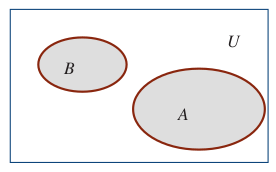
\includegraphics[width=0.6\linewidth]{/home/john/Documentos/MatematicasBioEstadisticaV1/BioestadisticaUnoUCES2021/images/FigUniona2} 

}

\caption{Relación de subconjunto [Imagen tomada de [@zill2012algebra] pág $32$]}\label{fig:FigUnionA-2}
\end{figure}
\begin{figure}

{\centering 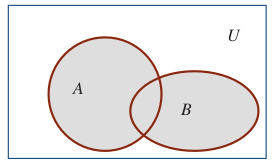
\includegraphics[width=0.6\linewidth]{/home/john/Documentos/MatematicasBioEstadisticaV1/BioestadisticaUnoUCES2021/images/FigUniona3} 

}

\caption{Relación de subconjunto [Imagen tomada de [@zill2012algebra] pág $32$]}\label{fig:FigUnionA-3}
\end{figure}

\hypertarget{propiedades-de-la-uniuxf3n}{%
\section{Propiedades de la Unión}\label{propiedades-de-la-uniuxf3n}}

\begin{figure}

{\centering 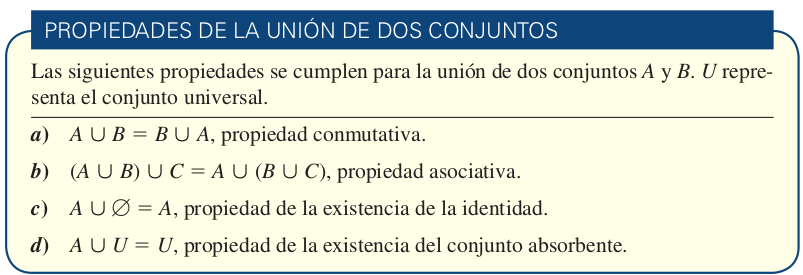
\includegraphics[width=0.6\linewidth]{/home/john/Documentos/MatematicasBioEstadisticaV1/BioestadisticaUnoUCES2021/images/PropiedadesUnion} 

}

\caption{Propiedades de la unión [Imagen tomada de [@zill2012algebra] pág $32$]}\label{fig:PropiedadesUnion}
\end{figure}

\begin{definition}
\protect\hypertarget{def:unnamed-chunk-29}{}{\label{def:unnamed-chunk-29} }La intersección de dos conjuntos \(A\) y \(B\) consta de todos los elementos que pertenecen a \(A\) y a \(B\). La intersección de \(A\) y \(B\) se denota por \(A \cap B\). {[}Tomado de \citep{zill2012algebra} pág \(30\){]}
\end{definition}

\[
A \cap B = \{ x | x \in A \ \text{y} \ x \in B\}
\]

\begin{figure}

{\centering 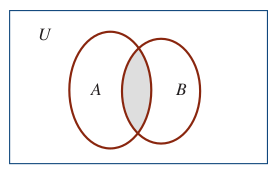
\includegraphics[width=0.6\linewidth]{/home/john/Documentos/MatematicasBioEstadisticaV1/BioestadisticaUnoUCES2021/images/FigInterseccion1} 

}

\caption{Intersección de conjuntos [Imagen tomada de [@zill2012algebra] pág $30$]}\label{fig:FigInterseccion}
\end{figure}

\hypertarget{propiedades-de-la-intersecciuxf3n}{%
\section{Propiedades de la Intersección}\label{propiedades-de-la-intersecciuxf3n}}

\begin{figure}

{\centering 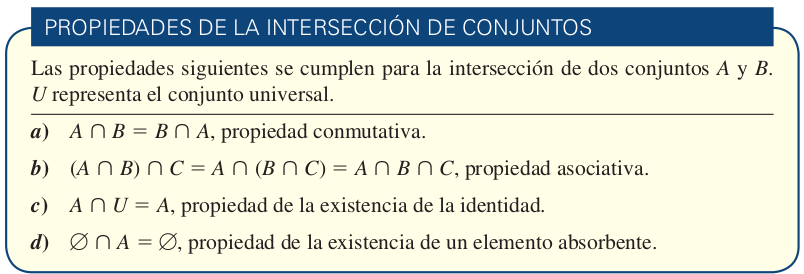
\includegraphics[width=0.6\linewidth]{/home/john/Documentos/MatematicasBioEstadisticaV1/BioestadisticaUnoUCES2021/images/PropiedadesInterseccion} 

}

\caption{Propiedades de la intersección [Imagen tomada de [@zill2012algebra] pág $30$]}\label{fig:PropiedadesInterseccion}
\end{figure}

\hypertarget{propiedades-de-la-uniuxf3n-y-la-intersecciuxf3n}{%
\section{Propiedades de la unión y la intersección}\label{propiedades-de-la-uniuxf3n-y-la-intersecciuxf3n}}

\begin{figure}

{\centering 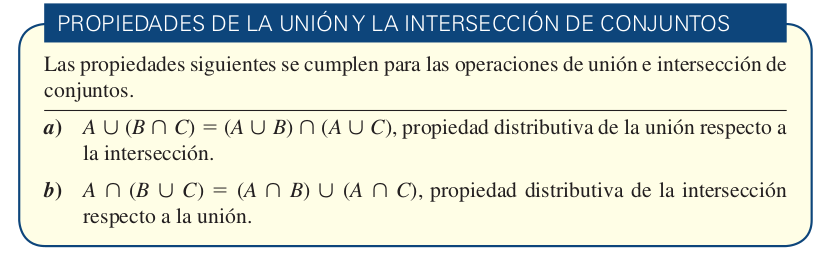
\includegraphics[width=0.6\linewidth]{/home/john/Documentos/MatematicasBioEstadisticaV1/BioestadisticaUnoUCES2021/images/FigUI} 

}

\caption{Propiedades de la unión y la intersección [Imagen tomada de [@zill2012algebra] pág $33$]}\label{fig:FigUI}
\end{figure}

\hypertarget{diferencia-entre-dos-conjuntos}{%
\section{Diferencia entre dos conjuntos}\label{diferencia-entre-dos-conjuntos}}

\begin{definition}
\protect\hypertarget{def:unnamed-chunk-30}{}{\label{def:unnamed-chunk-30} }La diferencia de dos conjuntos \(A\) y \(B\) consta de todos los elementos que pertenecen a \(A\) y no pertenecen a \(B\). La diferencia de \(A\) y \(B\) se denota por \(A - B\). {[}Tomado de \citep{zill2012algebra} pág \(34\){]}
\end{definition}

\[
A - B = \{ x | x \in A \ \text{y} \ x \notin B\}
\]

\begin{figure}

{\centering 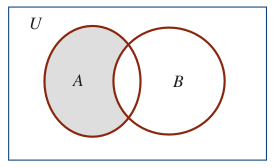
\includegraphics[width=0.6\linewidth]{/home/john/Documentos/MatematicasBioEstadisticaV1/BioestadisticaUnoUCES2021/images/FigDif} 

}

\caption{Diferencia entre conjuntos [Imagen tomada de [@zill2012algebra] pág $34$]}\label{fig:FigDif}
\end{figure}

\hypertarget{complemento-de-un-conjunto}{%
\section{Complemento de un conjunto}\label{complemento-de-un-conjunto}}

\begin{definition}
\protect\hypertarget{def:unnamed-chunk-31}{}{\label{def:unnamed-chunk-31} }El complemento de un conjunto \(A\) consta de todos los elementos del universo \(U\), y que no pertenecen a \(A\). El complemento de \(A\) se denota por \(A^{c}\). {[}Tomado de \citep{zill2012algebra} pág \(34\){]}
\end{definition}

\[
A'=A^{c} = \{ x | x \notin A \}
\]

\begin{figure}

{\centering 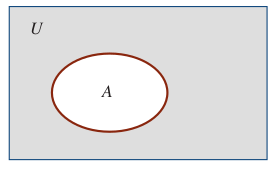
\includegraphics[width=0.6\linewidth]{/home/john/Documentos/MatematicasBioEstadisticaV1/BioestadisticaUnoUCES2021/images/FigComplemento} 

}

\caption{Complemento de un conjunto [Imagen tomada de [@zill2012algebra] pág $34$]}\label{fig:FigComplemento}
\end{figure}

\hypertarget{propiedades-del-algebra-de-conjuntos}{%
\section{Propiedades del algebra de conjuntos}\label{propiedades-del-algebra-de-conjuntos}}

\begin{figure}

{\centering 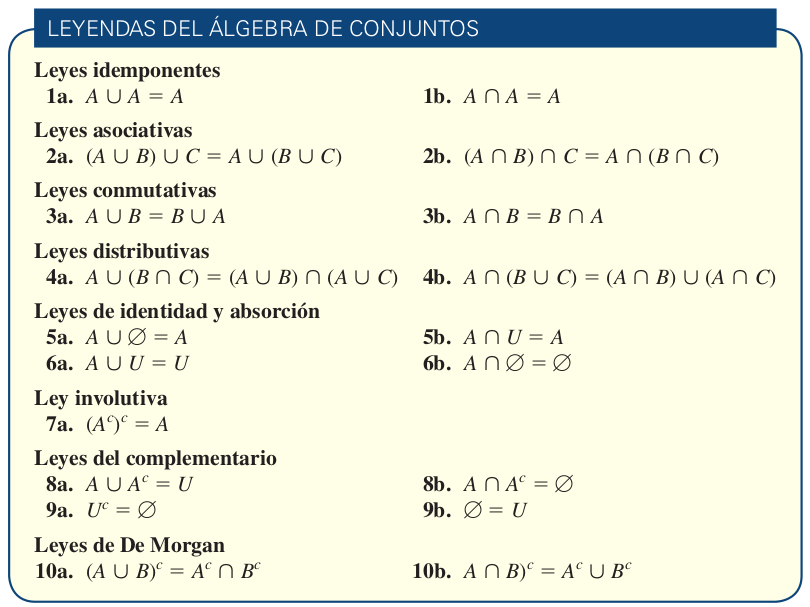
\includegraphics[width=0.6\linewidth]{/home/john/Documentos/MatematicasBioEstadisticaV1/BioestadisticaUnoUCES2021/images/FigPropiedadesGeneral} 

}

\caption{Leyes del algebra de Conjuntos [Imagen tomada de [@zill2012algebra] pág $36$]}\label{fig:FigPropiedadesGeneral}
\end{figure}

\hypertarget{ejemplo1}{%
\subsection{Ejemplo1}\label{ejemplo1}}

\begin{figure}

{\centering 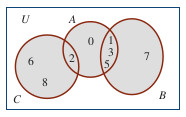
\includegraphics[width=0.6\linewidth]{/home/john/Documentos/MatematicasBioEstadisticaV1/BioestadisticaUnoUCES2021/images/EjemploConjuntos1} 

}

\caption{Ejemplo 1 de conjuntos [Imagen tomada de [@zill2012algebra] pág $33$]}\label{fig:FigEjConjunto1}
\end{figure}

A partir de la figura \ref{fig:FigEjConjunto1}, obtener la solución a los enunciados de conjuntos

\begin{itemize}
\item
  Obtener \(A \cup B=\{0, 2, 1, 3, 5, 7\}\)
\item
  Obtener \(A \cup C=\{0,2,6,8,1,3,5\}\)
\item
  Obtener \(C \cup B=?\)
\item
  Obtener \(A \cap B=?\)
\item
  Obtener \(A \cap C=?\)
\item
  Obtener \(C \cap B=?\)
\item
  Obtener \(A - B=?\)
\item
  Obtener \(B - A=\{7\}\)
\item
  Obtener \(A - C=?\)
\item
  Obtener \(C - B=?\)
\item
  Obtener \(B - C=?\)
\item
  Obtener \((A\cap B) - C=\{1,3,5\}\)
\item
  Obtener \((C\cap B) - A=?\)
\end{itemize}

\hypertarget{ejemplo2}{%
\subsection{Ejemplo2}\label{ejemplo2}}

\begin{figure}

{\centering 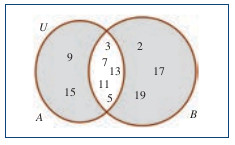
\includegraphics[width=0.6\linewidth]{/home/john/Documentos/MatematicasBioEstadisticaV1/BioestadisticaUnoUCES2021/images/EjemploConjuntos2} 

}

\caption{Ejemplo 2 de conjuntos [Imagen tomada de [@zill2012algebra] pág $35$]}\label{fig:FigEjConjunto2}
\end{figure}

A partir de la figura \ref{fig:FigEjConjunto2}, obtener la solución a los enunciados de conjuntos

\begin{itemize}
\item
  Obtener \(A \cup B=?\)
\item
  Obtener \(A \cap B=?\)
\item
  Obtener \(A - B=?\)
\item
  Obtener \(B - A=?\)
\end{itemize}

\hypertarget{ejemplo3}{%
\subsection{Ejemplo3}\label{ejemplo3}}

\begin{figure}

{\centering 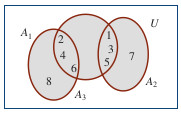
\includegraphics[width=0.6\linewidth]{/home/john/Documentos/MatematicasBioEstadisticaV1/BioestadisticaUnoUCES2021/images/EjemploConjuntos3} 

}

\caption{Ejemplo 3 de conjuntos [Imagen tomada de [@zill2012algebra] pág $33$]}\label{fig:FigEjConjunto3}
\end{figure}

A partir de la figura \ref{fig:FigEjConjunto3}, obtener la solución a los enunciados de conjuntos

\begin{itemize}
\item
  Obtener \({\bigcup}_{i=1}^{2}A_{i} =A_1 \cup A_2=\{8,6,4,2,1,3,5,7 \}\)
\item
  Obtener \({\bigcap}_{i=2}^{3}A_{i} =?\)
\item
  Obtener \({\bigcup}_{i=1}^{3}A_{i} =?\)
\item
  Obtener \({\bigcap}_{i=1}^{2}A_{i} =?\)
\item
  Obtener \({\bigcap}_{i=2}^{3}A_{i} =?\)
\item
  Obtener \({\bigcap}_{i=1}^{3}A_{i} =?\)
\item
  Obtener \(\left({\bigcup}_{i=1}^{2}A_{i}\right) - A_3=?\)
\item
  Obtener \(A_1-\left({\bigcup}_{i=2}^{3}A_{i}\right)=?\)
\end{itemize}

\hypertarget{conjuntos-numuxe9ricos}{%
\section{Conjuntos numéricos}\label{conjuntos-numuxe9ricos}}

\begin{figure}

{\centering 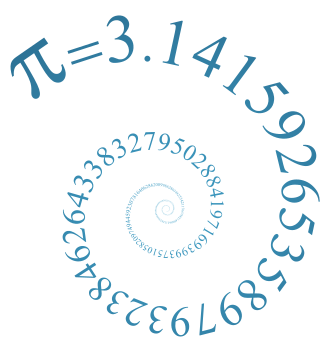
\includegraphics[width=4.61in]{/home/john/Documentos/MatematicasBioEstadisticaV1/BioestadisticaUnoUCES2021/images/FigPinumero} 

}

\caption{Número Irracional [Imagen tomada de [@zill2012algebra] pág $50$]}\label{fig:FigPinumero}
\end{figure}

\begin{definition}
\protect\hypertarget{def:unnamed-chunk-32}{}{\label{def:unnamed-chunk-32} }El conjunto de los números naturales consta de:
\end{definition}

\[
N=\{ 1,2,3,4,...\}
\]

\begin{definition}
\protect\hypertarget{def:unnamed-chunk-33}{}{\label{def:unnamed-chunk-33} }El conjunto de los números enteros consta de:
\end{definition}

\[
Z=\{...,-3,-2,-1,0,1,2,3,4,...\}
\]

\begin{definition}
\protect\hypertarget{def:unnamed-chunk-34}{}{\label{def:unnamed-chunk-34} }El conjunto de los números racionales consta de todos los números que son cociente de dos enteros, siempre que el denominador sea diferente de cero. Es decir:
\end{definition}

\[
Q=\{ \dfrac{p}{q} | p \ \text{y} \ q \ \ \text{son números enteros,} \ \ q \ \neq \ 0\}
\]
\begin{definition}
\protect\hypertarget{def:unnamed-chunk-35}{}{\label{def:unnamed-chunk-35} }El conjunto de los números irracionales consta de todos los números que no son el cociente de dos enteros, siempre que el denominador sea diferente de cero. Es decir:
\end{definition}

\[
Q^{*}=\{x |   \ x \neq \ \dfrac{p}{q}, \ \ q \ \neq \ 0\   \}
\]
\begin{definition}
\protect\hypertarget{def:unnamed-chunk-36}{}{\label{def:unnamed-chunk-36} }El conjunto de los números reales consta de la unión entre el conjunto de los racionales y los irracionales. Es decir:
\end{definition}

\[
R=\{x |   \ x \in Q \ \text{o} \ x \in Q^{*} \}=Q \cup Q^{*}
\]

\begin{figure}

{\centering 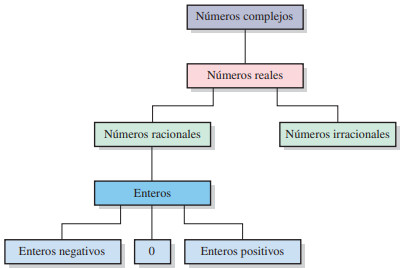
\includegraphics[width=0.6\linewidth]{/home/john/Documentos/MatematicasBioEstadisticaV1/BioestadisticaUnoUCES2021/images/EsquemaConjuntosReales1} 

}

\caption{Diagrama de los conjuntos numéricos [Imagen tomada de [@swokowski1996algebra] pág $3$]}\label{fig:FigConjuntoN}
\end{figure}

\hypertarget{propiedades-de-los-nuxfameros-reales}{%
\section{Propiedades de los números Reales}\label{propiedades-de-los-nuxfameros-reales}}

\begin{figure}

{\centering 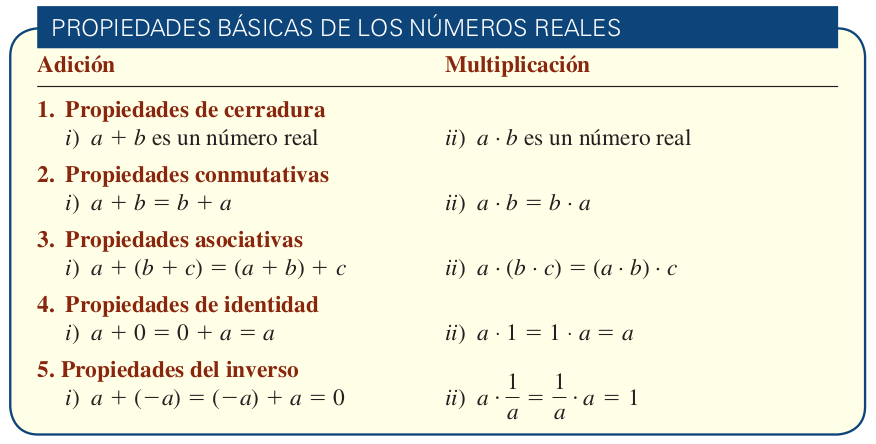
\includegraphics[width=0.6\linewidth]{/home/john/Documentos/MatematicasBioEstadisticaV1/BioestadisticaUnoUCES2021/images/FigPropiedadesReales} 

}

\caption{Propiedades de los números reales [Imagen tomada de [@zill2012algebra] pág $51$]}\label{fig:FigPropiedadesReales}
\end{figure}

\begin{figure}

{\centering 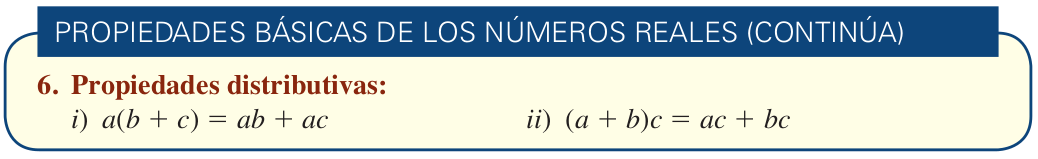
\includegraphics[width=0.6\linewidth]{/home/john/Documentos/MatematicasBioEstadisticaV1/BioestadisticaUnoUCES2021/images/FigPropiedadesRealesB} 

}

\caption{Propiedades de los números reales [Imagen tomada de [@zill2012algebra] pág $51$]}\label{fig:FigPropiedadesRealesB}
\end{figure}

\begin{figure}

{\centering 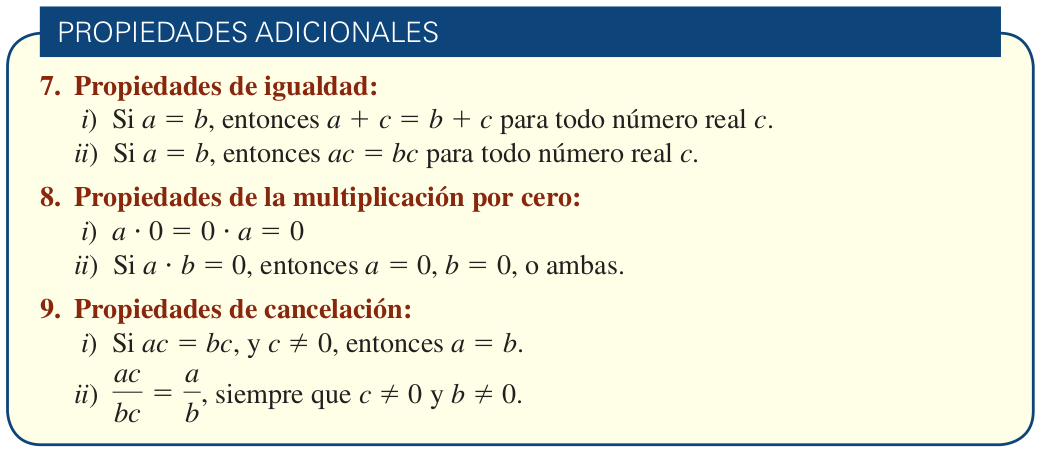
\includegraphics[width=0.6\linewidth]{/home/john/Documentos/MatematicasBioEstadisticaV1/BioestadisticaUnoUCES2021/images/FigPropiedadesRealesC} 

}

\caption{Propiedades de los números reales [Imagen tomada de [@zill2012algebra] pág $53$]}\label{fig:FigPropiedadesRealesC}
\end{figure}

\begin{figure}

{\centering 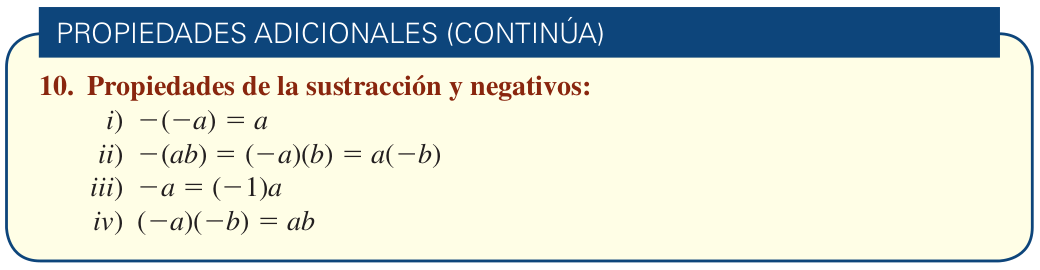
\includegraphics[width=0.6\linewidth]{/home/john/Documentos/MatematicasBioEstadisticaV1/BioestadisticaUnoUCES2021/images/FigPropiedadesRealesD} 

}

\caption{Propiedades de los números reales [Imagen tomada de [@zill2012algebra] pág $53$]}\label{fig:FigPropiedadesRealesD}
\end{figure}

\begin{figure}

{\centering 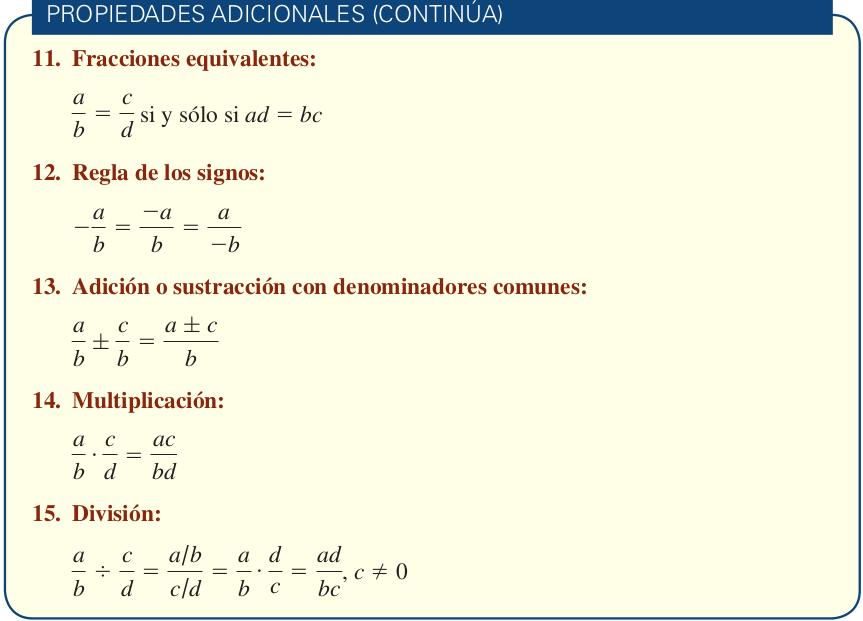
\includegraphics[width=0.6\linewidth]{/home/john/Documentos/MatematicasBioEstadisticaV1/BioestadisticaUnoUCES2021/images/FigPropiedadesRealesE} 

}

\caption{Propiedades de los números reales [Imagen tomada de [@zill2012algebra] pág $54$]}\label{fig:FigPropiedadesRealesE}
\end{figure}

\begin{figure}

{\centering 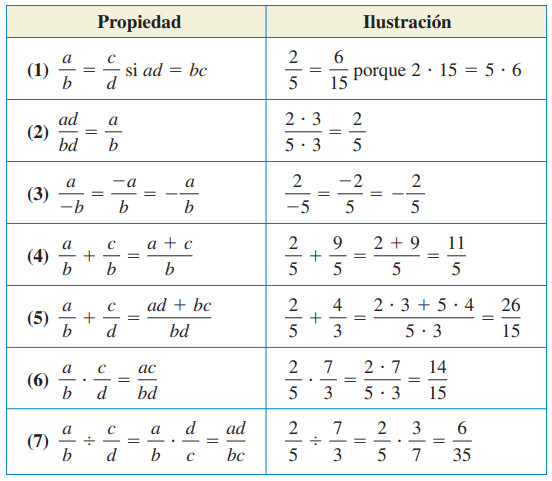
\includegraphics[width=0.6\linewidth]{/home/john/Documentos/MatematicasBioEstadisticaV1/BioestadisticaUnoUCES2021/images/PropiedadesFraccionarios1} 

}

\caption{Propiedades de los números reales [Imagen tomada de [@swokowski1996algebra] pág $8$]}\label{fig:FigPropiedadesRealesF1}
\end{figure}

\begin{figure}

{\centering 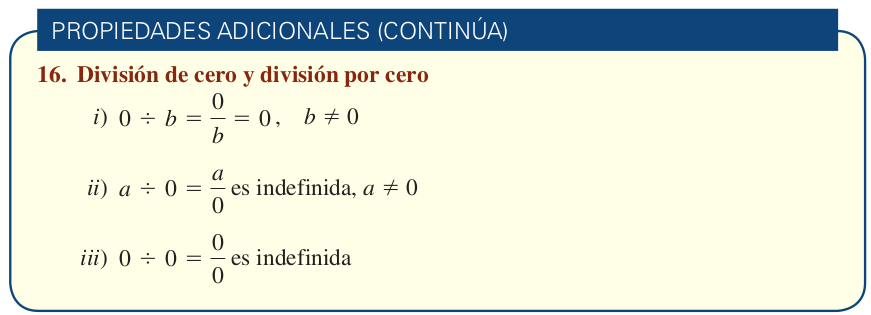
\includegraphics[width=0.6\linewidth]{/home/john/Documentos/MatematicasBioEstadisticaV1/BioestadisticaUnoUCES2021/images/FigPropiedadesRealesF} 

}

\caption{Propiedades de los números reales [Imagen tomada de [@zill2012algebra] pág $55$]}\label{fig:FigPropiedadesRealesF}
\end{figure}

\textbf{Podcast}

\hypertarget{conceptos-introductorios-de-probabilidad}{%
\section{Conceptos introductorios de probabilidad}\label{conceptos-introductorios-de-probabilidad}}

\begin{figure}

{\centering 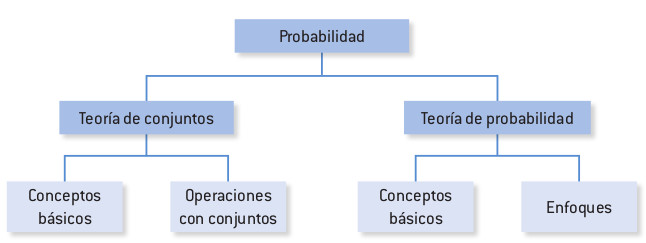
\includegraphics[width=0.6\linewidth]{/home/john/Documentos/MatematicasBioEstadisticaV1/BioestadisticaUnoUCES2021/images/ConjuntosT1} 

}

\caption{Esquema de probabilidad y conjuntos [Imagen tomada de [@zill2012algebra] pág $55$]}\label{fig:FigConjuntosT1}
\end{figure}

\begin{figure}

{\centering 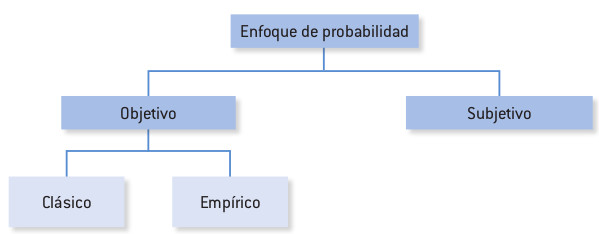
\includegraphics[width=0.6\linewidth]{/home/john/Documentos/MatematicasBioEstadisticaV1/BioestadisticaUnoUCES2021/images/ConjuntosT2} 

}

\caption{Esquema de probabilidad y conjuntos [Imagen tomada de [@zill2012algebra] pág $55$]}\label{fig:FigConjuntosT2}
\end{figure}

\begin{figure}

{\centering 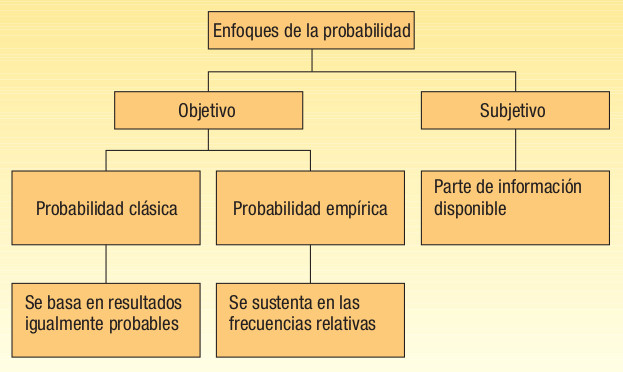
\includegraphics[width=0.6\linewidth]{/home/john/Documentos/MatematicasBioEstadisticaV1/BioestadisticaUnoUCES2021/images/ConjuntosT3} 

}

\caption{Esquema de probabilidad y conjuntos [Imagen tomada de [@zill2012algebra] pág $55$]}\label{fig:FigConjuntosT3}
\end{figure}

\begin{definition}
\protect\hypertarget{def:unnamed-chunk-37}{}{\label{def:unnamed-chunk-37} }Se dice que un espacio muestral \(S\) es discreto si su resultado puede ponerse en una correspondencia uno a uno con el conjunto de los enteros positivos
\end{definition}

\begin{definition}
\protect\hypertarget{def:unnamed-chunk-38}{}{\label{def:unnamed-chunk-38} }Un conjunto \(S\) que consta de todeos los resultados posibles de un experimento aleatorio se llama espacio muestal, y cada resultado se denomina punto muestral. Con frecuencia habrá más de un espacio muestral que puede describir los resultados de un experimento, pero generalmente habrá uno que provee la mayor información.
\end{definition}

\begin{definition}
\protect\hypertarget{def:unnamed-chunk-39}{}{\label{def:unnamed-chunk-39} }Se dice que un espacio muestral \(S\) es continuo si sus resultados consisten de un intervalo de números reales.
\end{definition}

\begin{definition}
\protect\hypertarget{def:unnamed-chunk-40}{}{\label{def:unnamed-chunk-40} }Un evento \(A\) del espacio muestral \(S\) es un grupo (ó subconjunto) de resultados contenidos en éste, cuyos miembros tiene una caracteríscita común.
\end{definition}

\begin{definition}
\protect\hypertarget{def:unnamed-chunk-41}{}{\label{def:unnamed-chunk-41} }Un evento es un subconjunto \(A\) del espacio muestral \(S\), es decir, un conjunto de resultados posibles. Si el resultado de un experimento es un elemento de \(A\), decimos que el evento \(A\) ocurrió. Un evento que consta de un punto sencillo de \(S\) se denomina con frecuencia un evento simple o elemental.
\end{definition}

\begin{definition}
\protect\hypertarget{def:unnamed-chunk-42}{}{\label{def:unnamed-chunk-42} }Sean \(S\) cualquier espacion muestral y \(A\) cualquier evento de éste. Se llamará función de probabilidad sobre el espacio muestral \(S\) a \(P(A)\) si satisface los siguientes axiomas:
\end{definition}

\hypertarget{definiciuxf3n1frecuentista}{%
\section{Definición1(Frecuentista)}\label{definiciuxf3n1frecuentista}}

Probabilidad empírica La probabilidad de que un evento ocurra representa una fracción de los eventos similares que sucedieron en el pasado.

Fórmula

\[
\text{Probabilidad empírica}=\dfrac{\text{Número de veces en que el evento ha ocurrido en el pasado}}{\text{Número total de observaciones}}
\]

\hypertarget{definiciuxf3n2cluxe1sica}{%
\section{Definición2(Clásica)}\label{definiciuxf3n2cluxe1sica}}

Probabilidad clasica La probabilidad clásica de un evento \(E\) se determina mediante la

Fórmula

\[
\text{Probabilidad clásica}=\dfrac{\text{Número de formas en las que puede ocurrir un evento}}{\text{Número total de posibles resultados}}
\]

La probabilidad clásica implica la determinación de la probabilidad de algún evento a priori (\textbf{antes del hecho})

\hypertarget{simulaciones-buxe1sicas}{%
\section{Simulaciones básicas}\label{simulaciones-buxe1sicas}}

\href{https://www.geogebra.org/m/cSfwCRkM}{Lanzamiento de un dado}

\href{https://www.geogebra.org/m/TwPXt2eD}{Lanzamiento de dos dados}

\href{https://www.geogebra.org/m/ZDNUEEwW}{Lanzamiento de una moneda}

\href{https://www.geogebra.org/m/nUZQCReV}{Lanzamiento de dos monedas}

\href{https://www.geogebra.org/m/z2cKzMwJ}{Lanzamiento de tres monedas}

\href{https://www.geogebra.org/m/pmxXRa55}{Lanzamiento de cuatro monedas}

\href{https://www.geogebra.org/m/MDXS6gVX}{Lanzamiento de un dado y una moneda}

\href{https://www.geogebra.org/m/kh2hSxsm}{Ley de los grandes números}

\hypertarget{lanzamiento-de-un-dado}{%
\section{Lanzamiento de un dado}\label{lanzamiento-de-un-dado}}

Lanzamiento de un dado

Espacio muestral

\[
S=\{1,2,3,4,5,6\}
\]

Evento : Subconjunto del espacio \(S\)

\[
A=\{2,4,6\}
\]

\[
B=\{1,3,5\}
\]

\hypertarget{lanzamiento-de-dos-dados}{%
\section{Lanzamiento de dos dados}\label{lanzamiento-de-dos-dados}}

Espacio muestral al lanzar dos dados

\[
S=\{(R1D=2,R2D=2);...\}
\]

Primera componente resultados del primer dado
Segunda componente resultados del segundo dado

\[
S=\{(2,2);(1,6);(1,3);(4,4);...\}
\]

Generar todas las posibles parejas al lanzar dos dados en forma inst.

Posibles Resultados de un dado (1):

\[
D1=\{1,2,3,4,5,6\}
\]

Posibles Resultados de un dado (2):

\[
D2=\{1,2,3,4,5,6\}
\]

las posibles parejas se realizan con el producto cartesiano

X=D1

Y=D2

\[
S=D1 \times D2=\{(1,1);(1,2);(1,3);(1,4);(1,5);(1,6);
(2,1);(2,2);(2,3);(2,4);(2,5);(2,6);...\}
\]

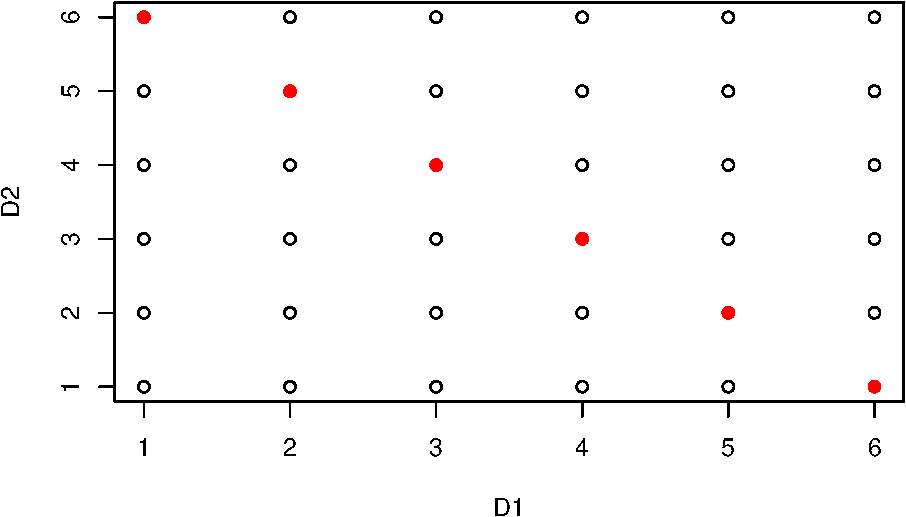
\includegraphics{BioestadisticaUnoUCES2021_files/figure-latex/unnamed-chunk-43-1.pdf}

Evento de los dados que al caer suman siete

\[
A=\{(1,6);(6,1);(2,5);(5,2);(3,4);(4,3)\}
\]

\hypertarget{lanzamiento-de-una-moneda-tres-veces}{%
\section{Lanzamiento de una moneda tres veces}\label{lanzamiento-de-una-moneda-tres-veces}}

\begin{figure}

{\centering 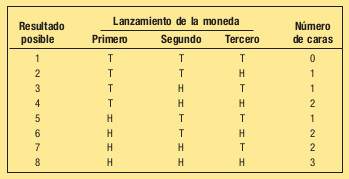
\includegraphics[width=0.6\linewidth]{/home/john/Documentos/MatematicasBioEstadisticaV1/BioestadisticaUnoUCES2021/images/Lanzamiento4veceUnaMoneda1} 

}

\caption{Tabla del lanzamiento de una moneda tres veces [Imagen tomada de [@zill2012algebra] pág $188$]}\label{fig:FigTablaMoneda1}
\end{figure}

\hypertarget{axioma-uno-de-la-probabilidad}{%
\section{Axioma Uno de la probabilidad}\label{axioma-uno-de-la-probabilidad}}

Para cualquier evento \(A\) contenido en el espacio de los resultados \(S\), se cumple que

\[P(A)\geq 0\]

\hypertarget{axioma-dos-de-la-probabilidad}{%
\section{Axioma Dos de la probabilidad}\label{axioma-dos-de-la-probabilidad}}

Si \(S\) es el conjunto que representa el espacio muestral de los resultados, entonces

\[P(S)=1\]

\hypertarget{axioma-tres-de-la-probabilidad}{%
\section{Axioma Tres de la probabilidad}\label{axioma-tres-de-la-probabilidad}}

Si para los eventos \(A_1,A_2,...,\) y \(A_i \cap A_j=\phi\) para toda \(i \neq j\), entonces

\begin{equation}
P(A_1 \cup A_2 \cup A_3 \cup...\cup A_k\cup...)=\\P(A_1)+P(A_2)+...+P(A_k)+...=\sum_{i=1}^{\propto}P(A_i)
\end{equation}

\hypertarget{teoremas-buxe1sicos-de-probabilidad}{%
\section{Teoremas básicos de probabilidad}\label{teoremas-buxe1sicos-de-probabilidad}}

\begin{theorem}
\protect\hypertarget{thm:TMA1-1}{}{\label{thm:TMA1-1} }Si \(A_1 \subset A_2\), entonces \(P(A_1) \leq P(A_2)\), y \(P(A_2-A_1)=P(A_2)-P(A_1)\)
\end{theorem}

\begin{theorem}
\protect\hypertarget{thm:TMA1-2}{}{\label{thm:TMA1-2} }Para todo evento \(A\)

\[0 \leq P(A) \leq 1\]

o sea, la probabilidad está entre \(0\) y \(1\)
\end{theorem}

\begin{theorem}
\protect\hypertarget{thm:TMA1-3}{}{\label{thm:TMA1-3} }\[ P(\Phi)=0 \]

es decir, el evento imposible tiene probabilidad cero.
\end{theorem}

\begin{theorem}
\protect\hypertarget{thm:TMA1-4}{}{\label{thm:TMA1-4} }Si \(A^{c}\) es el complemento de \(A\), entonces

\[P(A^{c})=1-P(A)\]
\end{theorem}

\begin{definition}
\protect\hypertarget{def:unnamed-chunk-44}{}{\label{def:unnamed-chunk-44} }Se dice que dos eventos \(A\) y \(B\) son mutumente excluyentes si no tienen resultados, o elementos comunes. En otras palabras los eventos \(A\) y \(B\) no pueden ocurrir al mismo tiempo.
\end{definition}

\begin{theorem}
\protect\hypertarget{thm:TMA1-5}{}{\label{thm:TMA1-5} }Si \(A=A_1\cup A_2... \cup A_n\), donde \(A_1\), \(A_2\), \(...\), \(A_n\) son mutuamente excluyentes, entonces

\[P(A)=P(A_1)+P(A_2)+...+P(A_n)=\sum_{i=1}^{n}P(A_i)\]
\end{theorem}

\begin{theorem}
\protect\hypertarget{thm:TMA1-6}{}{\label{thm:TMA1-6} }Si \(A\) y \(B\) son dos eventos cualesquiera, entonces

\[P(A \cup B)= P(A)+P(B)- P(A \cap B)\]
\end{theorem}

\begin{theorem}
\protect\hypertarget{thm:TMA1-7}{}{\label{thm:TMA1-7} }Para cualquier par de eventos \(A\) y \(B\),

\[P(A)=P(A \cap B)+P(A \cap B^{c})\]
\end{theorem}

\begin{theorem}
\protect\hypertarget{thm:TMA1-8}{}{\label{thm:TMA1-8} }Si un evento \(A\) debe dar como resultado la ocurrencia de uno de los eventos mutuamente excluyentes \(A_1\), \(A_2\),\ldots,\(A_n\), entonces

\[P(A)=P(A \cap A_1)+P(A \cap A_2) +...+ P(A \cap A_n)\]
\end{theorem}

\begin{theorem}
\protect\hypertarget{thm:TMA1-9}{}{\label{thm:TMA1-9} }Sean \(A\) y \(B\) dos eventos tales que \(P(A)>0\). Denótese por \(P(B|A)\) la probabilidad de \(B\) dado que ocurrió \(A\). Puesto que sabemos que ocurrió \(A\), éste se convierte en el nuevo espacio muestral reemplazando al original \(S\). A partir de esto llegamos a la definción

\[P(B|A)=\dfrac{P(A\cap B)}{P(A)}\]

\[P(A\cap B)=P(B|A)P(A)\]
\end{theorem}

\textbf{NOTA:} Para tres eventos cualesquiera \(A_1\), \(A_2\), \(A_3\), tenemos

\[P(A_1 \cap A_2 \cap A_3)=P(A_1)P(A_2|A_1)P(A_3| A_1 \cap A_2)\]

\begin{theorem}
\protect\hypertarget{thm:TMA1-10}{}{\label{thm:TMA1-10} }Si un evento \(A\) debe originar uno de los eventos mutuamente excluyentes \(A_1\), \(A_2\), \(...\), \(A_n\), entonces

\[P(A)=P(A_1)P(A|A_1)+P(A_2)P(A|A_2)+P(A_3)P(A|A_3)+...+P(A_n)P(A|A_n)\]
\end{theorem}

\begin{theorem}
\protect\hypertarget{thm:TMA1-11}{}{\label{thm:TMA1-11} }Suponga que \(A_1\), \(A_2\), \(...\), \(A_n\), son eventos mutuamente excluyentes cuya unión es el espacio muestral \(S\), es decir, que debe ocurrir uno de los eventos. Entonces si \(B\) es un evento cualquiera, tenemos

\[P(A_k|B)=\dfrac{P(A_k)P(B|A_k)}{\sum_{j=1}^{n}P(A_j)P(B|A_j)}\]

Esto nos permite encontrar las probabilidades de diferentes eventos \(A_1\), \(A_2\), \(...\), \(A_n\) que pueden hacer que ocurra \(B\).

Este teorema se conoce como el \textbf{teorema de Bayes} (ó el teorema de la probabilidad de las causas)
\end{theorem}

\begin{figure}

{\centering \includegraphics[width=0.4\linewidth]{/home/john/Documentos/MatematicasBioEstadisticaV1/BioestadisticaUnoUCES2021/images/TeoremaBayesUno} 

}

\caption{Teorema de Bayes [Imagen tomada de [@zill2012algebra] pág $51$]}\label{fig:FigTeoremaBayes}
\end{figure}

\hypertarget{demostraciuxf3n-probabilidad-del-complemento}{%
\section{Demostración probabilidad del complemento}\label{demostraciuxf3n-probabilidad-del-complemento}}

Demostrar que \(P(A^{c})=1-P(A)\)

Justificación (ó argumentación)

\[
\begin{split}
S &= A^{c} \cup A \\
P(S) &= P(A^{c} \cup A) \\
&= P(A^{c})+P(A), \ \ \ \ \ \text{ya que } A^{c} \cap A = \Phi\\
1 &= P(A^{c})+P(A), \ \ \ \ \ \text{ya que } P(S)=1\\
1-P(A) &= P(A^{c}), \ \ \ \ \ \text{Q.E.D. }
\end{split}
\]

\hypertarget{demostraciuxf3n-probabilidad-de-la-inclusiuxf3n}{%
\section{Demostración probabilidad de la inclusión}\label{demostraciuxf3n-probabilidad-de-la-inclusiuxf3n}}

Demostrar que si \(A \subseteq B\), entonces \(P(A) \leq P(B)\)

Justificación (ó argumentación)

\begin{figure}

{\centering \includegraphics[width=0.3\linewidth]{/home/john/Documentos/MatematicasBioEstadisticaV1/BioestadisticaUnoUCES2021/images/DMtma2} 

}

\caption{Justificación teorema 3.1 [Imagen tomada de [@zill2012algebra] pág $188$]}\label{fig:FigDMtma2}
\end{figure}

\[
\begin{split}
B &= A \cup (B-A) \\
P(B) &= P(A \cup (B-A)) \\
&= P(A)+P(B-A), \ \ \ \ \ \text{ya que } A \cap(B-A) = \Phi\\
\text{Luego, } P(A) &\leq  P(B), \ \ \ \ \ \text{Q.E.D. }
\end{split}
\]

\hypertarget{demostraciuxf3n-probabilidad-de-la-uniuxf3n}{%
\section{Demostración probabilidad de la unión}\label{demostraciuxf3n-probabilidad-de-la-uniuxf3n}}

Demostrar que \(P(A \cup B)=P(A)+P(B)-P(A \cap B)\)

Justificación (ó argumentación)

\begin{figure}

{\centering \includegraphics[width=0.3\linewidth]{/home/john/Documentos/MatematicasBioEstadisticaV1/BioestadisticaUnoUCES2021/images/DMtma3} 

}

\caption{Justificación teorema 3.6 [Imagen tomada de [@zill2012algebra] pág $188$]}\label{fig:FigDMtma3}
\end{figure}

\[
\begin{split}
A \cup B &= A \cup (B-A) \\
P(A \cup B) &= P\left( A \cup (B-A) \right) \\
P(A \cup B) &= P(A)+P(B-A), \ \ \ \ \ \text{ya que } A \cap(B-A) = \Phi\\
P(A \cup B) - P(A) &= P(B-A) \ \ \ \   (1)
\end{split}
\]

De otro lado

\begin{figure}

{\centering \includegraphics[width=0.3\linewidth]{/home/john/Documentos/MatematicasBioEstadisticaV1/BioestadisticaUnoUCES2021/images/DMtma3b} 

}

\caption{Justificación teorema 3.6 [Imagen tomada de [@zill2012algebra] pág $188$]}\label{fig:FigDMtma3b}
\end{figure}

\[
\begin{split}
B  &= (A \cap B)\cup (B-A)  \\
P(B)  &= P(A \cap B)+P(B-A), \ \ \ \ \ \text{ya que } A\cap B) \cap(B-A) = \Phi\\  \\
P(B) - P(A \cap B)   &= P(B-A) \ \ \ \ (2)
\end{split}
\]

de \((1)\) y \((2)\)

\[
\begin{split}
P(A \cup B) - P(A) &= P(B-A) \\
P(B) - P(A \cap B)   &= P(B-A) 
\end{split}
\]
Igualamos los lados izquierdos, así

\[
\begin{split}
P(A \cup B) - P(A) &= P(B) - P(A \cap B) \\
P(A \cup B) &= P(A)+P(B) - P(A \cap B), \ \ \ \ \ \text{Q.E.D. }
\end{split}
\]

\hypertarget{ejemplo-1}{%
\subsection{Ejemplo 1}\label{ejemplo-1}}

Suponga que lanzamos un dado justo una vez.

¿Qué probabilidad hay de obtener \(7\)?

\textbf{Respuesta}

Como el número \(7\) no está incluido en el conjunto \(S\) de todos los posibles resultados, el evento \(A\) de \textbf{obtener un \(7\)} es un evento imposible, es decir \(A=\Phi\). Entonces

\[
P(A)=P(\text{Obtener un 7})=\dfrac{0}{6}=0
\]

\hypertarget{ejemplo-2}{%
\subsection{Ejemplo 2}\label{ejemplo-2}}

Suponga que lanzamos un dado justo una vez.

¿Qué probabilidad hay de obtener un número menor que \(7\)?

\textbf{Respuesta}

Ya que el resultado de lanzar un dado son todos enteros positivos menores que \(7\), entonces el evento \(A\): \textbf{obtener un número menor que \(7\)} es

\[
A=\{1,2,3,4,5,6\}=S
\]

de donde

\[
P(A)=\dfrac{6}{6}=1
\]

\hypertarget{ejemplo-3}{%
\subsection{Ejemplo 3}\label{ejemplo-3}}

El 1 de febrero de 2003 explotó el transbordador espacial Columbia. Este fue el segundo desastre en 113 misiones espaciales de la NASA. Con base en esta información, cuál es la probabilidad de que una futura misión concluya con éxito?

\[
\text{Probabilidad de un vuelo exitoso}=\dfrac{111}{113}=0.98
\]

\hypertarget{ejemplo-4}{%
\subsection{Ejemplo 4}\label{ejemplo-4}}

Una encuesta de 34 estudiantes en una Universidad mostró que éstos tiene las siguientes especialidades:

\begin{enumerate}
\def\labelenumi{\arabic{enumi})}
\item
  Contabilidad 10
\item
  Finanzas 5
\item
  Economía 3
\item
  Administración 6
\item
  Marketing 10
\end{enumerate}

Suponga que elige a un estudiante y observa su especialidad.

Cuál es la probabilidad de que el estudiante tenga una especialidad en Administración?

Solución:

\[
\text{Probabilidad de que sea especialista en Administración}=\dfrac{6}{34}=\dfrac{3}{17}=0.18
\]

\begin{definition}
\protect\hypertarget{def:unnamed-chunk-45}{}{\label{def:unnamed-chunk-45} }Se dice que dos eventos \(A\) y \(B\) son mutumente excluyentes si no tienen resultados, o elementos comunes. En otras palabras los eventos \(A\) y \(B\) no pueden ocurrir al mismo tiempo.
\end{definition}

En términos de conjuntos, \(A\) y \(B\) son conjuntos \textbf{disjuntos} o \textbf{ajenos}; es decir,

\[
A \cap B=\Phi
\]

\hypertarget{regla-de-la-adiciuxf3n}{%
\section{Regla de la adición}\label{regla-de-la-adiciuxf3n}}

Para aplicar la regla de la adición, los eventos deben ser mutuamente excluyentes. Es decir si tenemos dos eventos son \(A\), y \(B\), estos son mutuamente excluyentes si su intersección es el vacío. Es decir

\[
A\cap B =\Phi
\]

\hypertarget{ejemplo3-1}{%
\subsection{Ejemplo3}\label{ejemplo3-1}}

Una máquina automática llena bolsas de plástico con una combinación de frijoles, brócoli y otras verduras. La mayoría de las bolsas contiene el peso correcto, aunque, como consecuencia de la variación del tamaño del frijol y de otras verduras, un paquete podría pesar menos o más. Una versión de \(4000\) paquetes que se llenaron el mes pasado arrojó los siguientes datos:

Cuál es la probabilidad de que un paquete en particular pese menos o pese más?

\begin{Shaded}
\begin{Highlighting}[]
\NormalTok{Peso <-}\StringTok{ }\KeywordTok{c}\NormalTok{(}\StringTok{"Menos peso"}\NormalTok{,}\StringTok{"Peso satisfactorio"}\NormalTok{,}\StringTok{"Más peso"}\NormalTok{)}
\NormalTok{Evento <-}\StringTok{ }\KeywordTok{c}\NormalTok{(}\StringTok{"A"}\NormalTok{,}\StringTok{"B"}\NormalTok{,}\StringTok{"C"}\NormalTok{)}
\NormalTok{Numero_Paquetes <-}\StringTok{ }\KeywordTok{c}\NormalTok{(}\DecValTok{10}\NormalTok{,}\DecValTok{3600}\NormalTok{,}\DecValTok{300}\NormalTok{)}
\NormalTok{Probabilidad <-}\StringTok{ }\KeywordTok{c}\NormalTok{(}\FloatTok{0.025}\NormalTok{,}\FloatTok{0.900}\NormalTok{,}\FloatTok{0.075}\NormalTok{)}

\NormalTok{Ejemplo <-}\StringTok{ }\KeywordTok{data.frame}\NormalTok{(Peso, Evento, Numero_Paquetes, Probabilidad)}

\NormalTok{knitr}\OperatorTok{::}\KeywordTok{kable}\NormalTok{(}
\NormalTok{Ejemplo , }\DataTypeTok{caption =} \StringTok{'Tabla en Frecuencia para Datos Agrupados'}\NormalTok{,}
  \DataTypeTok{booktabs =} \OtherTok{TRUE}
\NormalTok{)}
\end{Highlighting}
\end{Shaded}

\begin{table}

\caption{\label{tab:Tabla10}Tabla en Frecuencia para Datos Agrupados}
\centering
\begin{tabular}[t]{llrr}
\toprule
Peso & Evento & Numero\_Paquetes & Probabilidad\\
\midrule
Menos peso & A & 10 & 0.025\\
Peso satisfactorio & B & 3600 & 0.900\\
Más peso & C & 300 & 0.075\\
\bottomrule
\end{tabular}
\end{table}

Solución: Como \(A\) y \(C\) son eventos excluyentes, entonces \(A\cap C=\Phi\), ya que un paquete de verduras mixtas no puede pesar menos, tener el peso satisfactorio y pesar más al mismo tiempo.

\[
P(A \ \text{ó} \ C)=P(A\cup C)=P(A)+P(C)
\]

\[
P(A\cup C)=P(A)+P(C)=0.025+0.075=0.10
\]

\begin{definition}
\protect\hypertarget{def:unnamed-chunk-46}{}{\label{def:unnamed-chunk-46} }Se dice que dos eventos \(A\) y \(B\) son independientes, si \(P(B|A)=P(B)\). Es decir, la probabilidad de que ocurra \(B\) no está afectada por la ocurrencia o no de \(A\). Además esto equivale a:

\[P(A \cap B)=P(A)P(B)\]
\end{definition}

\begin{definition}
\protect\hypertarget{def:unnamed-chunk-47}{}{\label{def:unnamed-chunk-47} }Una tabla de contingencia es cuadro que se utiliza para clasificar observaciones de una muestraa de acuerdo con dos o más características identificables.
\end{definition}

\begin{figure}

{\centering \includegraphics[width=0.8\linewidth]{/home/john/Documentos/MatematicasBioEstadisticaV1/BioestadisticaUnoUCES2021/images/EsquemaProbabilidad2} 

}

\caption{Esquema de probabilidad conjunta [Imagen tomada de [@zill2012algebra] pág $188$]}\label{fig:FigEsquema2}
\end{figure}

\hypertarget{ley-de-los-grandes-nuxfameros}{%
\section{Ley de los grandes números}\label{ley-de-los-grandes-nuxfameros}}

En una gran cantidad de intentos, la probabilidad empírica de un evento se aproxima a su probabilidad real.

\begin{figure}

{\centering \includegraphics[width=0.6\linewidth]{/home/john/Documentos/MatematicasBioEstadisticaV1/BioestadisticaUnoUCES2021/images/TABLALeyGrandesN1} 

}

\caption{Tabla ley de los grandes números [Imagen tomada de [@zill2012algebra] pág $188$]}\label{fig:FigTABLALeyGn1}
\end{figure}

\hypertarget{tabla-de-contingencia}{%
\section{Tabla de contingencia}\label{tabla-de-contingencia}}

\begin{figure}

{\centering \includegraphics[width=0.4\linewidth]{/home/john/Documentos/MatematicasBioEstadisticaV1/BioestadisticaUnoUCES2021/images/TABLA3P} 

}

\caption{Tabla de contingencia definiciones básicas [Imagen tomada de [@zill2012algebra] pág $188$]}\label{fig:FigTABLA3P}
\end{figure}

La tabla describe la relación entre dos eventos \(A\) y \(B\). Para obtener \(P(A_{j})\) se debe proceder como:

\[
    P(A_{j})=\sum_{i=1}^{2}\frac{n_{ij}}{n}
\]

Ejemplo

La tabla de contingencia muestra la relación entre el color de cabello del pelo y el color de ojos de un grupo de \(1770\) hombres alemanes.

\begin{figure}

{\centering \includegraphics[width=0.6\linewidth]{/home/john/Documentos/MatematicasBioEstadisticaV1/BioestadisticaUnoUCES2021/images/TABLA2P} 

}

\caption{Tabla de contingencia realción del color de cabello y color de ojos [Imagen tomada de [@zill2012algebra] pág $188$]}\label{fig:FigTABLA2P}
\end{figure}

\[
j=1,j=2 \\
p(A_j)=\sum_{i=1}^2\dfrac{n_{ij}}{n}=\dfrac{n_{1j}}{n}+\dfrac{n_{2j}}{n}=\dfrac{n_{1j}+n_{2j}}{n}\\
p(A_1)=\sum_{i=1}^2\dfrac{n_{i1}}{n}=\dfrac{n_{11}}{n}+\dfrac{n_{21}}{n}=\dfrac{n_{11}+n_{21}}{n}\\
p(A_2)=\sum_{i=1}^2\dfrac{n_{i2}}{n}=\dfrac{n_{12}}{n}+\dfrac{n_{22}}{n}=\dfrac{n_{12}+n_{22}}{n}\\
p(A_3)=\sum_{i=1}^2\dfrac{n_{i3}}{n}=\dfrac{n_{13}}{n}+\dfrac{n_{23}}{n}=\dfrac{n_{13}+n_{23}}{n}
\]

\begin{figure}

{\centering \includegraphics[width=0.4\linewidth]{/home/john/Documentos/MatematicasBioEstadisticaV1/BioestadisticaUnoUCES2021/images/TABLA3P} 

}

\caption{Tabla de contingencia definiciones básicas [Imagen tomada de [@zill2012algebra] pág $188$]}\label{fig:FigTABLA3Pa}
\end{figure}

La tabla describe la relación entre dos eventos \(A\) y \(B\). Para obtener \(P(B_{i})\) se debe proceder como:

\[
    P(B_{i})=\sum_{j=1}^{2}\frac{n_{ij}}{n}
\]

\[
i=1,i=2\\
p(B_i)=\sum_{j=1}^2\dfrac{n_{ij}}{n}=\dfrac{n_{i1}}{n}+\dfrac{n_{i2}}{n}=\dfrac{n_{i1}+n_{i2}}{n}\\
p(B_1)=\sum_{j=1}^2\dfrac{n_{1j}}{n}=\dfrac{n_{11}}{n}+\dfrac{n_{12}}{n}=\dfrac{n_{11}+n_{12}}{n}\\
p(B_2)=\sum_{j=1}^2\dfrac{n_{2j}}{n}=\dfrac{n_{21}}{n}+\dfrac{n_{22}}{n}=\dfrac{n_{21}+n_{22}}{n}\\
p(B_3)=\sum_{j=1}^2\dfrac{n_{3j}}{n}=\dfrac{n_{31}}{n}+\dfrac{n_{32}}{n}=\dfrac{n_{31}+n_{32}}{n}\\
\]

\begin{figure}

{\centering \includegraphics[width=0.4\linewidth]{/home/john/Documentos/MatematicasBioEstadisticaV1/BioestadisticaUnoUCES2021/images/TABLA3P} 

}

\caption{Tabla de contingencia definiciones básicas [Imagen tomada de [@zill2012algebra] pág $188$]}\label{fig:FigTABLA3Pb}
\end{figure}

La tabla describe la relación entre dos eventos \(A\) y \(B\). Para obtener \(P(A_{j}\cap B_{i})\) se debe proceder como:

\[
    P(A_{j}\cap B_{i})=\frac{n_{ij}}{n}
\]

\begin{equation}
P(A_j\cap B_i)=\dfrac{n_{ij}}{n}\\
i=1,j=1\\
P(A_1\cap B_1)=\dfrac{n_{11}}{n}
\end{equation}

\begin{equation}
P(A_2\cap B_2)=\dfrac{n_{22}}{n}
\end{equation}

\begin{Shaded}
\begin{Highlighting}[]
\NormalTok{nal <-}\StringTok{ }\DecValTok{400}\OperatorTok{/}\DecValTok{1770}
\KeywordTok{round}\NormalTok{(nal,}\DecValTok{2}\NormalTok{)}\OperatorTok{*}\DecValTok{100}
\end{Highlighting}
\end{Shaded}

\begin{verbatim}
## [1] 23
\end{verbatim}

La tabla describe la relación entre dos eventos \(A\) y \(B\). Para obtener \(P(B_{i} | A_{j})\) se debe proceder como:

\[
    \dfrac{P(B_{i}\cap A_{j})}{P(A_{j})}=P(B_{i} | A_{j})=\dfrac{n_{ij}}{\sum_{i=1}^{2}n_{ij}}
\]

\[
    \dfrac{P(B_{i=1}\cap A_{j=2})}{P(A_{j=2})}=P(B_{1} | A_{2})=\dfrac{n_{ij}}{\sum_{i=1}^{2}n_{ij}}=\dfrac{n_{12}}{n_{12}+n_{22}}
\]

\begin{equation}
i=1,2\\
j=1,2,3\\
P(A_j\cap B_i)=\dfrac{n_{ij}}{n}\\
i=1;j=1\\
P(A_1\cap B_1)=\dfrac{n_{11}}{n}\\
P(\text{ojos castaños y cabello castaño})=P(A_1\cap B_1)=\dfrac{n_{11}}{n}=\dfrac{400}{1770}\\
P(\text{ojos castaños y cabello rojo})=P(A_3\cap B_1)=\dfrac{n_{13}}{n}=\dfrac{20}{1770}\\
\end{equation}

\hypertarget{ejemploencuesta-de-ver-cine}{%
\subsection{Ejemplo(Encuesta de ver cine)}\label{ejemploencuesta-de-ver-cine}}

Ejemplo

Una encuesta de \(150\) adultos clasificados según su género y la cantidad de películas que vieron cine el mes pasado.

\begin{figure}

{\centering \includegraphics[width=0.6\linewidth]{/home/john/Documentos/MatematicasBioEstadisticaV1/BioestadisticaUnoUCES2021/images/TABLA1P} 

}

\caption{Tabla de contingencia de películas según el genero [Imagen tomada de [@zill2012algebra] pág $188$]}\label{fig:FigTABLA1P}
\end{figure}

Cúal es la probabilidad de que no se vió ninguna película

donde:

\begin{enumerate}
\def\labelenumi{\arabic{enumi})}
\item
  \(B_1\): Cero películas
\item
  \(B_2\): Una sola película
\item
  \(B_3\): Dos o más películas
\item
  \(n\): Tamaño de la muestra es de \(150\) personas
\item
  \(A_1\): Hombres
\item
  \(A_2\): Mujeres
\end{enumerate}

\begin{Shaded}
\begin{Highlighting}[]
\NormalTok{n<-}\StringTok{ }\DecValTok{150}
\NormalTok{numB1 <-}\StringTok{ }\DecValTok{60}
\NormalTok{rd1 <-}\StringTok{ }\KeywordTok{round}\NormalTok{(numB1}\OperatorTok{/}\NormalTok{n,}\DecValTok{2}\NormalTok{)}
\end{Highlighting}
\end{Shaded}

\[P(B_1)=\dfrac{60}{150}=0.4\]

\begin{Shaded}
\begin{Highlighting}[]
\NormalTok{n<-}\StringTok{ }\DecValTok{150}
\NormalTok{numB2 <-}\StringTok{ }\DecValTok{70}
\NormalTok{rd2 <-}\StringTok{ }\KeywordTok{round}\NormalTok{(numB2}\OperatorTok{/}\NormalTok{n,}\DecValTok{2}\NormalTok{)}
\end{Highlighting}
\end{Shaded}

\[P(B_2)=\dfrac{70}{150}=0.47\]

\begin{Shaded}
\begin{Highlighting}[]
\NormalTok{n<-}\StringTok{ }\DecValTok{150}
\NormalTok{numB3 <-}\StringTok{ }\DecValTok{70}
\NormalTok{rd3 <-}\StringTok{ }\KeywordTok{round}\NormalTok{(numB3}\OperatorTok{/}\NormalTok{n,}\DecValTok{2}\NormalTok{)}
\end{Highlighting}
\end{Shaded}

\[P(B_3)=\dfrac{70}{150}=0.47\]

\begin{Shaded}
\begin{Highlighting}[]
\NormalTok{n <-}\StringTok{ }\DecValTok{150}
\NormalTok{numA1 <-}\StringTok{ }\DecValTok{70}
\NormalTok{rd4 <-}\StringTok{ }\KeywordTok{round}\NormalTok{(numA1}\OperatorTok{/}\NormalTok{n,}\DecValTok{2}\NormalTok{)}
\end{Highlighting}
\end{Shaded}

\[
P(A_1)=\dfrac{70}{150}= 0.47
\]

\begin{Shaded}
\begin{Highlighting}[]
\NormalTok{n <-}\StringTok{ }\DecValTok{150}
\NormalTok{numA2 <-}\StringTok{ }\DecValTok{80}
\NormalTok{rd5 <-}\StringTok{ }\KeywordTok{round}\NormalTok{(numA2}\OperatorTok{/}\NormalTok{n,}\DecValTok{2}\NormalTok{)}
\end{Highlighting}
\end{Shaded}

\[
P(A_2)=\dfrac{80}{150}= 0.53
\]

\begin{Shaded}
\begin{Highlighting}[]
\NormalTok{n <-}\StringTok{ }\DecValTok{150}
\NormalTok{numB3A2 <-}\StringTok{ }\DecValTok{10}
\NormalTok{rd6 <-}\StringTok{ }\KeywordTok{round}\NormalTok{(numB3A2}\OperatorTok{/}\NormalTok{n,}\DecValTok{2}\NormalTok{)}
\end{Highlighting}
\end{Shaded}

\[
P(A_2\cap B_3)=\dfrac{10}{150}= 0.07
\]

\hypertarget{probabilidad-condicional-y-tabla-de-contingencia}{%
\section{Probabilidad condicional y tabla de contingencia}\label{probabilidad-condicional-y-tabla-de-contingencia}}

Probabilidad condicional

Si tenermos dos eventos \(A\), \(B\)

siempre que \(P(A)>0\) y \(P(B)>0\), entonces

\begin{equation}
P(A|B)=\dfrac{P(A\cap B)}{P(B)}\\
P(B|A)=\dfrac{P(A\cap B)}{P(A)}
\end{equation}

\begin{equation}
P(A\cap B)=P(A).P(A|B)
\end{equation}

\begin{equation}
P(A\cap B)=P(B).P(B|A)
\end{equation}

\hypertarget{ejemplocafuxe9}{%
\subsection{Ejemplo(Café)}\label{ejemplocafuxe9}}

\begin{figure}

{\centering \includegraphics[width=0.6\linewidth]{/home/john/Documentos/MatematicasBioEstadisticaV1/BioestadisticaUnoUCES2021/images/GRAFICAtabladeContingencia3} 

}

\caption{Tabla de contingencia de películas segun el genero [Imagen tomada de [@zill2012algebra] pág $188$]}\label{fig:FigTABLA4P}
\end{figure}

GRAFICAtabladeContingencia3

\begin{enumerate}
\def\labelenumi{\arabic{enumi})}
\item
  \(B_1\): Menos de 30
\item
  \(B_2\): Entre 30 a 40
\item
  \(B_3\): Entre 40 a 50
\item
  \(B_4\): 50 ó más
\item
  \(n\): Tamaño de la muestra es de \(150\) personas
\item
  \(A_1\): Bajo
\item
  \(A_2\): Moderado
\item
  \(A_3\): Alto
\end{enumerate}

\[
P(B_3|A_2)=\dfrac{P(B_3\cap A_2)}{P(A_2)}=\dfrac{\dfrac{24}{300}}{\dfrac{110}{300}}=\dfrac{24}{110}
\]

\hypertarget{regla-del-producto}{%
\section{Regla del producto}\label{regla-del-producto}}

Dados dos eventos \(A\) y \(B\), diremos que son independientes uno del otro si cumplen que

\[
P(A|B)=P(A) \ \ \ \text{ó} \ \ \ P(B|A)=P(B)
\]
Entonces se puede deducir la \textbf{regla del producto} para la probabilidad de la intersección entre dos eventos \(A\) y \(B\).

\[
P(A\cap B)=P(A).P(B|A)\\
P(A\cap B)=P(A).P(B)
\]

\hypertarget{teorema-de-bayes}{%
\section{Teorema de Bayes}\label{teorema-de-bayes}}

Dado su interés en las matemáticas, intentó crear una fórmula para llegar a la probabilidad de que Dios existiera sobre la base de la evidencia de la que, se disponía en la Tierra. Más tarde, Pierre-Simon Laplace perfeccionó el trabajo de Bayes y le dio el nombre de teorema de Bayes. De una forma entendible.

Ejemplo(Urnas)

\begin{figure}

{\centering \includegraphics[width=0.6\linewidth]{/home/john/Documentos/MatematicasBioEstadisticaV1/BioestadisticaUnoUCES2021/images/Problema3UrnasV1} 

}

\caption{Teorema de Bayes problema de las Urnas [Imagen tomada de [@zill2012algebra] pág $51$]}\label{fig:FigTeoremaBayes2}
\end{figure}

Tenemos tres urnas:

La urna \(A\) con 3 bolas rojas y 5 negras, la urna \(B\) con 2 bolas rojas y 1 negra, y la urna \(C\) con 2 bolas rojas y 3 negras. Escoger una urna al azar y extraemos una bola. Si la bola ha sido roja, ¿cual es la probabilidad de haber sido extraída de la urna \(A\)?

\[
    P(A|R)=\dfrac{P(A)P(R|A)}{P(A)P(R|A)+P(B)P(R|B)+P(C)P(R|C)}
\]

\[
    P(A|R)=\dfrac{(\frac{1}{3})(\frac{3}{8})}{(\frac{1}{3})(\frac{3}{8})+(\frac{1}{3})(\frac{2}{3})+(\frac{1}{3})(\frac{2}{5})}=\dfrac{45}{173}=0.260
\]

Ejemplo(CIRUGIAS)

Un médico cirujano se especializa en cirugías estéticas. Entre sus pacientes, el 20 por ciento se realizan correcciones faciales, un 35 por ciento implantes mamarios y el restante en otras cirugías correctivas. Se sabe además, que son de genero masculino el 25 por ciento de los que se realizan correcciones faciales, 15 por ciento implantes mamarios y 40 por ciento otras cirugías correctivas. Si se selecciona un paciente al azar, determine:

\begin{itemize}
\tightlist
\item
  La probabilidad de que sea de género masculino.
\end{itemize}

*Si resulta que es de genero masculino, determine la probabilidad que se haya realizado una cirugía de implantes mamarios.

\begin{itemize}
\item
  \(F\): Pacientes que realizan cirugías faciales
\item
  \(M\): Pacientes que se realizan implantes mamarios
\item
  \(O\): Pacientes que se realizan otras cirugías correctivas
\item
  \(H\): pacientes de género masculino
\end{itemize}

\[
S=F\cup M \cup O
\]
\[H=(H\cap F)\cup (H\cap M) \cup (H\cap O)\]

\[
P(H)=?\\
P(H)=P((H\cap F)\cup (H\cap M) \cup (H\cap O))\\
\]

\[
    P(H)=P(F)P(H|F)+P(M)P(H|M)+P(O)P(H|O)
\]

\[
    P(H)=(0.2)(0.25)+(0.35)(0.15)+(0.45)(0.40)=0.28
\]

\[
P(H)=P(H\cap F)+ P(H\cap M)+ P(H\cap O)=0.28\\
P(H\cap F)=P(F)P(H|F)\\
P(Mujer)=1-P(H)=1-0.28
\]

\[
    P(M|H)=\dfrac{P(M)P(H|M)}{P(M)P(H|M)+P(F)P(H|F)+P(O)P(H|O)}
\]

\[
    P(M|H)=\dfrac{(0.35)(0.15)}{(0.35)(0.15)+(0.2)(0.25)+(0.45)(0.40)}=\dfrac{0.0525}{0.2825}=0.19
\]

Ejemplo(Máquinas de productos)

\begin{figure}

{\centering \includegraphics[width=0.6\linewidth]{/home/john/Documentos/MatematicasBioEstadisticaV1/BioestadisticaUnoUCES2021/images/Problema3MaquinasV1} 

}

\caption{Teorema de Bayes problema de las máquinas [Imagen tomada de [@zill2012algebra] pág $51$]}\label{fig:FigTeoremaBayes3}
\end{figure}

Tres máquinas, \(A\),\(B\) y \(C\), producen el \(45\) porciento, \(30\) porciento y \(25\) porciento, respectivamente, del total de las piezas producidas en una fábrica. Los porcentajes de producción defectuosas de estas máquinas son del \(3\) porciento, \(4\) porciento y \(5\) porciento. Tomamos, al azar, una pieza y resulta ser defectuosa; calcular la probabilidad de haber sido producida por al máquina \(B\).

\[
    P(B|D)=\dfrac{P(B)P(D|B)}{P(A)P(D|A)+P(B)P(D|B)+P(C)P(D|C)}
\]

\[
    P(B|D)=\dfrac{(0.30)(0.04)}{(0.30)(0.04)+(0.45)(0.03)+(0.25)(0.05)}=\dfrac{12}{38}=0.316
\]

\hypertarget{modelos-de-probabilidad}{%
\chapter{Modelos de probabilidad}\label{modelos-de-probabilidad}}

\hypertarget{temas-extras}{%
\chapter{Temas Extras}\label{temas-extras}}

\hypertarget{programaciuxf3n-r_rstudio}{%
\chapter{Programación R\_Rstudio}\label{programaciuxf3n-r_rstudio}}

\hypertarget{repaso-de-r-y-rstudio}{%
\section{Repaso de R y Rstudio}\label{repaso-de-r-y-rstudio}}

Los conceptos básicos para el manejo de R los recorremos usando el documento elaborado por Vicente Coll y Pedro J Pérez (Junio 2017) \href{https://www.uv.es/pjperez/curso_R/tt_2_conceptos_basicos_R.html}{Página web}

Ver también la página web \href{https://r-coder.com/inicio/}{Todo sobre programción en R}

\hypertarget{puxe1ginas-donde-se-puede-trabajar-r-en-luxednea}{%
\section{Páginas donde se puede trabajar R en línea}\label{puxe1ginas-donde-se-puede-trabajar-r-en-luxednea}}

Una página donde se puede elaborar prácticas básicas para uso de comandos en R es: \href{https://www.tutorialspoint.com/execute_r_online.php}{Compile R online}

También se puede trabajar en línea con las siguientes páginas.

\begin{itemize}
\item
  \href{https://rdrr.io/snippets/}{R en línea Dos}
\item
  \href{https://paiza.io/es/projects/new}{R en línea Tres}
\item
  \href{https://www.mycompiler.io/new/r}{R en línea Cuatro}
\end{itemize}

\hypertarget{videos-de-clase}{%
\chapter{Videos de Clase}\label{videos-de-clase}}

\hypertarget{clases-semestre-02-2021}{%
\section{Clases semestre 02-2021}\label{clases-semestre-02-2021}}

\href{https://ucesedu-my.sharepoint.com/:v:/g/personal/jestrada_ces_edu_co/EcW4-ARUR_pAle6_zBnBtGoBdYWSsPRCVFZQszjdWHFzjA?e=ZK3UQ9}{Clase1 Miércoles 14 de Julio 2021}

\href{https://ucesedu-my.sharepoint.com/:v:/g/personal/jestrada_ces_edu_co/EQoVbUGbrmJEowXESb6CpicB0JEoonbDN9-VdOZnuj976w?e=u3r92I}{Clase2 Viernes 16 de Julio 2021}

\href{https://ucesedu-my.sharepoint.com/:v:/g/personal/jestrada_ces_edu_co/Ee6nFXz-reVFoTFQLAsBjxcBNweX4cgLZnRUVp9fv1aPlg?e=uF5o1O}{Clase3 Miércoles 21 de Julio 2021}

{[}Clase4 Viernes 23 de Julio 2021 PROBLEMAS DE RED NO SE REALIZO LA CLASE{]}

\href{https://ucesedu-my.sharepoint.com/:v:/g/personal/jestrada_ces_edu_co/EUgB9cGyPQlLlgfg8_niKpMB4xU4fVxQTwFIhuVlgF72vg?e=zDxSIF}{Clase5 Miércoles 28 de Julio 2021}

\href{https://ucesedu-my.sharepoint.com/:v:/g/personal/jestrada_ces_edu_co/Eaw1mCf-FY5GiW86uhnjfb0BcZcBcFJTxLqP7fNS_Xxwxw?e=rdgPDa}{Clase6 Viernes 30 de Julio 2021}

\href{https://ucesedu-my.sharepoint.com/:v:/g/personal/jestrada_ces_edu_co/EWVsuXTmL7pOrYhTfQUK1JUBJduPXmi_MQARUBSnBGbwDg?e=Ndsv9N}{Clase7 Miércoles 04 de Agosto 2021}

\href{https://ucesedu-my.sharepoint.com/:v:/g/personal/jestrada_ces_edu_co/ESRTE_mdbwVFtZIrK319T2gBTsBRjddWSzbzDZVkrp-4ag?e=pBhMKE}{Clase8 Viernes 06 de Agosto 2021}

\hypertarget{videos-de-asesoruxeda}{%
\chapter{Videos de Asesoría}\label{videos-de-asesoruxeda}}

\hypertarget{asesoruxedas-semestre-02-2021}{%
\section{Asesorías semestre 02-2021}\label{asesoruxedas-semestre-02-2021}}

  \bibliography{book.bib,packages.bib}

\end{document}
